\documentclass{tudelft-report}

\usepackage{comment}
\usepackage{todonotes}
\usepackage{amssymb}

\usepackage{pifont}
\newcommand{\xmark}{\ding{55}}

%% Set up the bibliography
\usepackage[style=apa]{biblatex}
\addbibresource{report.bib}

%% Colour box for lemma's
\usepackage[most]{tcolorbox}
\tcbset{
  colback=orange!10,      % light orange background
  colframe=orange!80!black, % darker orange border
  coltitle=black,         % title colour
  fonttitle=\bfseries\large, % bold and slightly larger title
  boxrule=0.5mm,          % border thickness
  arc=2mm,                % corner radius
  top=1mm, bottom=1mm, left=2mm, right=2mm,
}


%% Additional packages and commands
\usepackage{parskip}
\setlist{itemsep=-2pt} % Reducing white space in lists slightly
\renewcommand{\deg}{\si{\degree}\xspace} % Use \deg easily, everywhere

%% ----------------------------------------------------------------------
%%    Begin of document + Frontmatter (Roman page numbering)
%% ----------------------------------------------------------------------

\begin{document}

\frontmatter

%% Define the main parameters
\title{Robust rocket landing through reinforcement learning.}
\subtitle{Developing Robust and Adaptive Policies for Rocket Descent and Landing.}
\author{Jonathan Robert van Zyl}

\subject{MSc Thesis, Faculty of Aerospace Engineering, Control and Operations} % Cover only
\affiliation{Delft University of Technology} % Cover only
\coverimage{figures/Covers/cover1.jpg} % Aspect ratio of 2:3 (portrait) recommended
\definecolor{title}{HTML}{4884d6} % Color for cover title

\makecover

\begin{titlepage}

\begin{center}

%% Print the title
{\makeatletter
\largetitlestyle\fontsize{45}{45}\selectfont\@title
\makeatother}

%% Print the subtitle
{\makeatletter
\ifdefvoid{\@subtitle}{}{\bigskip\titlestyle\fontsize{20}{20}\selectfont\@subtitle}
\makeatother}

\bigskip
\bigskip

by

\bigskip
\bigskip

%% Print the name of the author
{\makeatletter
\largetitlestyle\fontsize{25}{25}\selectfont\@author
\makeatother}

\bigskip
\bigskip

%% Print table with names and student numbers
\setlength\extrarowheight{2pt}
\begin{tabular}{lc}
    Student Name & Student Number \\\midrule
    Jonathan van Zyl & 5039738 \\
\end{tabular}

\vfill

%% Print some more information at the bottom
\begin{tabular}{ll}
    Cover Image Source: & \cite{mars_rocket_image} \\
    Supervisors: & Dr.ir.E van Kampen \\
    Project Duration: & November, 2024 - July, 2025 \\
    Faculty: & Faculty of Aerospace Engineering, Delft
\end{tabular}

\bigskip
\bigskip

\begin{comment}
%% Add a source and description for the cover and optional attribution for the template
\begin{tabular}{p{15mm}p{10cm}}
    Cover: & Canadarm 2 Robotic Arm Grapples SpaceX Dragon by NASA under CC BY-NC 2.0 (Modified) \\
    % Feel free to remove the following attribution, it is not required - still appreciated :-)
    Style: & TU Delft Report Style, with modifications by Daan Zwaneveld
\end{tabular}
\end{comment}

\end{center}

%% Insert the TU Delft logo at the bottom of the page
\begin{tikzpicture}[remember picture, overlay]
    \node[above=10mm] at (current page.south) {%
        
\includegraphics{figures/logo-black}
    };
\end{tikzpicture}

\end{titlepage}


\chapter*{Preface}
\addcontentsline{toc}{chapter}{Preface}

\emph{To make space more accessible, launch costs must be reduced. Consequently, companies are moving towards reusable launch vehicles. Consider, for example, how impractical it would be to scrap an aircraft after every flight—flying would become prohibitively expensive. However, research into applying reinforcement learning to address this issue remains limited, hence the motivation for this thesis.
}

\emph{On a personal note, this Thesis allowed me to cap off 5 years of studying at TU Delft. I decided on Aerospace Engineering during high school due to a curiosity about rockets and space exploration. Through my bachelors I developed interests in machine learning and particularly reinforcement learning. Following this, my interests in controls spiked during a year as a controls engineer at Forze. Rockets, controls and reinforcement learning are the main pillars of this thesis; and I think I am very privileged to have worked on a project for 9 months of which I like the topics so much.
}

\emph{I would like to thank my supervisor Dr. ir. Erik-Jan van Kampen for his support and advice, without which I would have been lost. Secondly, I extend my thanks to all the lecturers who have taught me.}

\emph{During this thesis I realised that most essential knowledge is acquired in the first 2 years of the bachelors. So simply put, my advice to all students wishing to pursue becoming aerospace engineers is: attend your lectures.
}

\begin{flushright}
{\makeatletter\itshape
    \@author \\
    Delft, \monthname{} \the\year{}
\makeatother}
\end{flushright}

\tableofcontents
\listoffigures
\listoftables

\chapter*{Nomenclature}
\addcontentsline{toc}{chapter}{Nomenclature}

\section*{Abbreviations}

\begin{longtable}{p{2.5cm}p{12cm}}
    \toprule
    Abbreviation & Definition \\
    \midrule\endhead % Add abbreviations alphabetically here:
    ACS & Aerodynamic Control Surface \\ %YES
    AIL & Adversarial Imitation Learning \\ %YES
    ARL & Adversarial Reinforcement Learning \\ %YES
    ARPL & Adversarially Robust Policy Learning \\ %YES
    A2C & Advantage Actor-Critic \\ %YES
    A3C & Asynchronous Advantage Actor-Critic \\ %YES
    BC & Behavioural Cloning \\ %YES
    BNN & Bayesian Neural Network \\ % YES
    CoG & Centre of Gravity \\ %YES
    CoP & Centre of Pressure \\ %YES
    DDP & Deterministic Policy Gradient \\ %YES
    DDPG & Deep Deterministic Policy Gradient \\ %YES
    DDRL & Deep Distributed Reinforcement Learning \\ %YES
    DGPS & Differential Global Positioning System \\ %YES
    DoF & Degree of Freedom \\ %YES - moved to introduction
    DP & Dynamic Programming \\ %YES - twice first in probform
    DQN & Deep Q-learning \\ %YES
    D4PG & Distributed Distributional Deterministic Policy Gradients \\ %YES
    EA & Evolutionary Algorithms \\ %YES
    ES & Evolutionary Strategies \\ %YES
    FADS & Flush Air Data System \\ %YES
    GA & Genetic Algorithm \\ %YES
    GAIL & Generative Adversarial Imitation Learning \\ %YES
    Gorila & General RL Architecture \\ %YES
    GNC & Guidance, Navigation and Control \\ %YES
    GNSS & Global Navigation Satellite System \\ %YES
    HER & Hindsight Experience Replay \\ %YES
    ICM & Intrinsic Curiosity Module \\ %YES
    ICS & Intelligent Control Systems \\ %YES
    IMPALA & Importance Weighted Actor Learner Architecture \\ %YES
    IMS & Inertial Measurement Unit \\ %YES
    IRL & Inverse Reinforcement Learning \\ %YES
    ISA & International Standard Atmosphere \\ %YES
    JAX & A programming language called JAX \\ %YES
    KL & Kullback-Leiber \\ %not referenced, but needed
    Mars-GRAM & Mars Global Reference Atmospheric Model \\ %YES
    MARL & Multi-Agent Reinforcement Learning \\ %YES
    MC & Monte Carlo \\ %YES - moved to introduction
    MIMO & Multiple-Input Multiple-Output \\ %YES
    MPC & Model Predictive Control \\ %YES
    MPO & Maximum a posteriori Policy Optimisation \\ %YES
    MSE & Mean Squared Error \\ %YES
    MVM & Main Valve Management \\ %YES
    OU & Ornstein-Uhlenbeck \\ %YES
    PER & Prioritised Experience Replay \\ %YES
    PNN & Progressive Neural Network \\ %YES
    PPO & Proximal Policy Optimisation \\ %YES - moved to introduction
    PSN & Parameter space noise \\ %YES
    PWIL & Primal Wasserstein Imitation Learning \\ %YES
    QARL & Quantal Adversarial RL \\ %YES
    RARL & Robust Adversarial Reinforcement Learning \\ %YES
    RARARL & Risk Averse RARL \\ %YES
    RCS & Reaction Control System \\ %YES
    RL & Reinforcement Learning \\ %YES
    RND & Random Network Distillation \\ %YES
    SAC & Soft Actor-Critic \\ %YES
    SARSA & State-Action-Reward-State-Action \\ %YES
    SCvx & Successive Convexification \\ %YES
    SGD & Stochastic Gradient Descent \\ %YES
    SLSQP & Sequential Least Squares Programming \\ %YES
    SOCP & Second Order Cone Programming \\ %YES
    SQIL & Soft W Imitation Learning \\ %YES
    TD & Temporal Difference \\ %YES - twice, first in probform
    TD3 & Twin Delay Deep Deterministic Policy Gradient \\ %YES
    TVC & Thrust Vectoring Control \\ %YES
    TRPO & Trust Region Policy Optimisation \\ %YES
    VMPO & On-policy MPO \\ %YES
    WBS & Work Breakdown Structure \\ %YES - appendix
    \bottomrule
\end{longtable}

\section*{Symbols}

\subsection*{Reinforcement Learning}

\begin{longtable}{p{2.5cm}p{12cm}}
    \toprule
    Symbol & Definition \\
    \midrule\endhead
    % Symbols with no units:
    $a$ & Action \\
    $A(s, a)$ & Advantage stream \\
    $\hat{a}(s_t, s_{t+1})$ & Action prediction \\
    $\tilde{a}$ & Gaussian-noise modified action \\
    $|\mathcal{A}|$ & Total number of available actions \\
    $\hat{A}$ & Advantage estimate \\
    $D_{KL}$ & KL divergence  \\
    $D_w$ & Discriminator network (GAIL)\\
    $e_{TD}$ & Temporal difference error \\
    $\mathbb{E}$ & Expectation \\
    $G$ & Monte Carlo return \\
    $\mathcal{H}$ & Entropy \\
    $\mathcal{H}^{\text{target}}$ & Target entropy \\
    $I$ & Identity matrix \\
    $\mathcal{L}$ & Loss function \\
    $M^X$ & Trust region threshold for "X" \\
    $\mathcal{N}$ & Gaussian distribution \\
    $N^{\text{buffer}}$ & Buffer size \\
    $\tilde{p}$ & Priority \\
    $P$ & Probability \\
    $Q(s,a)$ & Action-value function \\
    $Q^{*}(s,a)$ & Optimal action-value function \\
    $Q_Z$ & Distributional critic \\
    $\hat{Q}$ & Risk modified Q-value \\
    $R(s, a)$ & Expected rewards \\
    $R^{\text{intrinsic}}$ & Intrinsic rewards \\
    $\mathcal{R}$ & Replay buffer \\
    $s$ & State \\
    $V(s)$ & Value stream \\
    $w$ & Network's weights \\
    $y_{X}$ & Network "X's" output \\
    
    \midrule
    $\alpha$ & Learning Rate \\
    $\alpha^V$ & Value stream learning rate \\
    $\alpha_{\text{PER}}$ & PER hyperparameter controller importance of sampling previous transitions with a higher reward probability\\
    $\beta_{\text{PER}}$ & PER hyperparameter determining correction between faster learning and bias correction\\
    $\gamma$ & Discount factor \\
    $\epsilon$ & Sampled Gaussian noise \\
    $\epsilon^{\text{PPO}}$ & PPO KL constraint bound \\
    $\epsilon^V$ & Hyperparameter for control of variance in weights (MPO) \\
    $\zeta$ & Actor network \\
    $\zeta_S$ & Stochastic actor network \\
    $\eta$ & Intrinsic reward scaling factor (ICM) \\
    $\theta$ & Network's parameters \\
    $\tilde{\theta}$ & Gaussian altered network parameters \\
    $\theta_{A}$ & Advantage stream's parameters (duelling Q-networks) \\
    $\theta_{V}$ & Value stream's parameters (duelling Q-networks) \\
    $\theta^{\mu}$ & Actor's parameters \\
    $\theta^{-}$ & Target network's parameters \\
    $\kappa_A$ & Risk-seeking hyperparameter (RARARL) \\
    $\kappa_P$ & Risk-aversion hyperparameter (RARARL) \\
    $\lambda^X$ & Lagrangian multiplier of "X" \\
    $\nu$ & Temperature hyperparameter \\
    $\nu^*$ & Optimal temperature hyperparameter \\
    $\pi$ & Policy \\
    $\sigma$ & Standard deviation \\
    $\bar{\tau}$ & Target network update weight \\
    $\phi$ & State features \\
    $\hat{\phi}$ & Predicted state features \\
    \bottomrule
\end{longtable}

\subsection*{Simulation and rocket landing control}


\begin{longtable}{p{2.5cm}p{12cm}}
    \toprule
    Symbol & Definition \\
    \midrule\endhead
    a & Acceleration [m/s\textsuperscript{2}] \\
    $\mathbf{a}_{S}$ & \textit{Starship} action space [-] \\
    $\mathbf{a}_{\text{superheavy}}$ & Super heavy action space [-] \\
    $c_{fl}$ & Pendulum's damping coefficient [kgm/s] \\
    $C_d$ & Drag coefficient [-] \\
    $C_{d,0}$ & Zero-lift drag coefficient [-] \\
    $C_l$ & Lift coefficient [-] \\
    $C_m$ & Aerodynamic pitching coefficient [-] \\
    $C_n$ & Aerodynamic yawing coefficient [-] \\
    $C_p$ & Aerodynamic rolling coefficient [-] \\
    $C_y$ & Side-force coefficient [-] \\
    $d$ & Distance between rocket CoG and fluid's [m] \\
    $d^{\text{tank}}$ & Distance between rocket's CoG and the tanks [m] \\
    $D$ & Drag [N] \\
    $F$ & Force [N] \\
    $g$ & Gravitational acceleration [m/s\textsuperscript{2}] \\
    $g_0$ & Gravitational acceleration at sea level [m/s\textsuperscript{2}] \\
    $h$ & Altitude [m] \\
    $h_f$ & Fuel height [m] \\
    $H^{\text{tank}}$ & Tank's height [m] \\
    $I$ & Moment of inertia [kg/m\textsuperscript{2}] \\
    $\mathbf{I}_r$ & Rocket's inertia matrix excluding tanks [kg/m\textsuperscript{2}] \\
    $\mathbf{I}_{fl}$ & Tank's fluid's inertia matrix [kg/m\textsuperscript{2}] \\
    $I_{sp}$ & Specific impulse [m/s] \\
    $k_d$ & Induced drag factor [-] \\
    $k_{fl}$ & Pendulum's spring constant [kg/s\textsuperscript{2}] \\
    $l$ & Pendulum's length [m] \\
    $L$ & Lift [N] \\
    $L_l$ & Lagrangian [J] \\
    $LG$ & Landing gear deployment [binary] \\
    $m$ & Mass [kg] \\
    $\dot{m}$ & Mass flow [kg/s] \\
    $m_f(t)$ & Fuel and Oxidiser mass at time "t" [kg]\\
    $m_{\text{dry}}(t)$ & Dry mass at time "t" [kg] \\
    $m_{\text{fuel}}(t)$ & Fuel  mass at time "t" [kg]\\
    $m_{\text{fl}}(t)$ & Tank's fluid  mass at time "t" [kg]\\
    $m_{\text{oxidiser}}(t)$ & Fuel  mass at time "t" [kg]\\
    $m_{\text{wet}}(t)$ & Dry mass at time "t" [kg] \\
    $m_r$ & Rocket mass excluding tank(s) i.e. dry mass [kg] \\
    $M$ & Moment [Nm] \\
    $M_a$ & Aerodynamic pitching moment [Nm] \\
    $N_a$ & Aerodynamic yawing moment [Nm] \\
    $N_{ACS}$ & Number of aerodynamic control surfaces [-] \\
    $N_C$ & Number of fixed hot-gas thrusters [-] \\
    $N_{RCS}$ & Number of fixed cold gas thrusters [-] \\
    $N_{TVC}$ & Number of torque vectored thrusters [-] \\
    $p$ & Roll rate [rad/s] \\
    $P_a$ & Aerodynamic rolling moment [Nm] \\
    $q$ & Quaternion component [-] \\
    $\hat{q}$ & Generalised coordiante of Lagrangian [-] \\
    $Q$ & Cost weight matrix penalising state deviation (MPC) [-] \\
    $\hat{Q}$ & Generalised force [-] \\
    $\hat{r}$ & Radial unit vector [-] \\
    $\vec{r}$ & Position vector (x,y,z) [m] \\
    $R$ & Cost weight matrix penalising control effort (MPC) [-] \\
    $R_{\text{Earth}}$ & Earth's radius [m] \\
    $R_f$ & Ratio of oxidiser to fuel mass flow [-] \\
    $R^{\text{tank}}$ & Tank's radius [m] \\
    $\vec{s}$ & Pendulum's displacement from origin vector [m] \\
    $S$ & Area [m\textsuperscript{2}] \\
    $t$ & Time [s] \\
    $T_i$ & Thrust for engine $i$ [N] \\
    $T_l$ & Kinetic energy [J] \\
    $u_j$ & RCS thruster $j$ state (on/off) [-] \\
    $v$ & Velocity component [m/s] \\
    $v_{\text{rel}}$ & Reltive velocity component [m/s] \\
    $V$ & Volume [m\textsuperscript{3}] \\
    $V_l$ & Potential energy [J] \\
    $x$ & Position coordinate (Cartesian) [m] \\
    $y$ & Position coordinate (Cartesian) [m] \\
    $z$ & Position coordinate (Cartesian) [m] \\
    \midrule
    $\alpha$ & Angle of attack [rad] \\
    $\beta$ & Sideslip angle [rad] \\
    $\gamma$ & Flight path angle [rad] \\
    $\delta_k$ & Deflection angle of aerodynamic control surface $k$ [rad] \\
    $\theta$ & Pitch angle (Euler) [rad] \\
    $\theta_{fl}$ & Fluid's polar angle (spherical) [rad] \\
    $\theta_i$ & Pitch thrust vector angle for engine $i$ (Euler)[rad] \\
    $\vec{\Theta}_{fl}$ & Fluid's angle vector (spherical) [rad] \\
    $\rho$ & Atmospheric density [kg/m\textsuperscript{3}] \\
    $\phi$ & Roll angle (Euler) [rad] \\
    $\phi_{fl}$ & Fluid's azimuth angle  (spherical) [rad] \\
    $\psi$ & Yaw angle (Euler) [rad] \\
    $\psi_i$ &  Yaw thrust vector angle for engine $i$ [rad] \\
    $\omega$ & Angular velocity component [rad/s] \\
    $\vec{\omega}_{fl}$ & Tank's fluids angular velocity vector [rad/s] \\
    $\vec{\omega}_{r}$ & Rockets angular velocity vector i.e. \(\vec{\omega}\) [rad/s] \\
    $\mathbf{\Omega(\omega)}$ & Quaternion kinematics matrix [-] \\
    \bottomrule
\end{longtable}


%% ----------------------------------------------------------------------
%%    Mainmatter (Arabic page numbering)
%% ----------------------------------------------------------------------

\mainmatter

\chapter{Introduction}
\label{chp:introduction}
\input{mainmatter/Introduction/0_Introduction}

\section{Hypothesis}
\label{sec:hypothesis}
\input{mainmatter/Introduction/1_Hypothesis}

\section{Research questions}
\label{sec:research_questions}
\input{mainmatter/Introduction/2_ResearchQuestions}

\section{Desired success and evaluation metrics}
\label{sec:metrics}
\input{mainmatter/Introduction/3_Metrics}

\section{Project Planning}
\label{sec:project_planning}
\input{mainmatter/Introduction/4_ProjectPlanning}

\section{Novelty of the project}
\label{sec:novelty}
\input{mainmatter/Introduction/5_Novelty}



\section{Hypothesis}
\label{sec:hypothesis}
\begin{center}
    \textbf{Reinforcement learning can replace current control systems for the rocket landing problem. This results in a more robust, adaptive, and computationally efficient solution for online use.}
\end{center}

Robustness is defined in this work as the minimum performance for the control system to function in a practical environment (\cite{ZHANG201041}). Robust control design results in stable controls within bounded modelling errors and uncertainties. As a data driven controller cannot have stability proven through classical methods. This study defines the outcome as robust if above minimum required performance is given in terms of accuracy under environmental disturbances, defined in \autoref{sec:metrics}. Future work can extend this to other disturbances like static parameter variations and sensor noise.

\section{Research questions}
\label{sec:research_questions}
This section defines the project research questions; they are written to answer the hypothesis of \autoref{sec:hypothesis}, with the metrics used to determine success denoted later in \autoref{sec:metrics}.

\begin{tcolorbox}[title={\textbf{Research question 1}}]
How can data-driven control systems be effectively applied for a rocket’s high-level trajectory planning and mid-level guidance control during landing?
\end{tcolorbox}

\begin{tcolorbox}[title={\textbf{Research question 2}}]
What factors affect the computational feasibility of mimicking traditional trajectory planning methods, like convex optimisation, through a learnt policy?
\end{tcolorbox}

\begin{tcolorbox}[title={\textbf{Research question 3}}]
What level of fidelity is needed for a simulation model to provide a conceptual study into policy transferability?
\end{tcolorbox}

% Flight phase characteristics?

\section{Desired success and evaluation metrics}
\label{sec:metrics}
The rocket landing control system shall be evaluated in three main categories: \textbf{robustness}, \textbf{accuracy} and \textbf{safety}.

\begin{center}
    \textbf{System failure}: the inability to meet the safety and accuracy requirements would result in a rocket crash.
\end{center}


\textbf{FILL IN AFTER ACTUALLY HAVE A LANDING WORKING!}

\section{Project Planning}
\label{sec:project_planning}


New project planning include:
a) Research phase I and II
b) Work breakdown structure
c) Gantt chart
d) Risk analysis

\section{Novelty of the project}
\label{sec:novelty}
This work expands the study of using reinforcement learning for rocket landing. The key novelties are:
\begin{enumerate}
    \item Imitation learning to mimic a convex optimiser, Model Predictive Controller (MPC), for trajectory planning can prove advantageous over end-to-end learning as it may result in improved sample efficiency. Secondly, it can be used in the learnt policy, which can be improved after mimicking the MPC's solution. Finally, the solution will be more computationally efficient than traditional trajectory planning methods, like loss-less convexification for optimisation, explained in \autoref{sec:landing_control}.
    \item A hierarchal intelligent controller structure, through splitting up the high-level trajectory planner and mid-level guidance layer for a modular design.
    \item A novel reinforcement learning algorithm, as described in \autoref{sec:off_policy_on_line_RL}, combining the best features of traditional reinforcement learning for an online, off-policy and model-free approach.
    \item Use robust reinforcement learning techniques to test the learnt policies' robustness thoroughly.
    \item Modelling of fuel sloshing provides a complex environment with needed dynamics to validate the workings of the controller. The majority of studies neglect fuel sloshing.
\end{enumerate}



\section{Hypothesis}
\label{sec:hypothesis}
\begin{center}
    \textbf{Reinforcement learning can replace current control systems for the rocket landing problem. This results in a more robust, adaptive, and computationally efficient solution for online use.}
\end{center}

Robustness is defined in this work as the minimum performance for the control system to function in a practical environment (\cite{ZHANG201041}). Robust control design results in stable controls within bounded modelling errors and uncertainties. As a data driven controller cannot have stability proven through classical methods. This study defines the outcome as robust if above minimum required performance is given in terms of accuracy under environmental disturbances, defined in \autoref{sec:metrics}. Future work can extend this to other disturbances like static parameter variations and sensor noise.

\section{Research questions}
\label{sec:research_questions}
This section defines the project research questions; they are written to answer the hypothesis of \autoref{sec:hypothesis}, with the metrics used to determine success denoted later in \autoref{sec:metrics}.

\begin{tcolorbox}[title={\textbf{Research question 1}}]
How can data-driven control systems be effectively applied for a rocket’s high-level trajectory planning and mid-level guidance control during landing?
\end{tcolorbox}

\begin{tcolorbox}[title={\textbf{Research question 2}}]
What factors affect the computational feasibility of mimicking traditional trajectory planning methods, like convex optimisation, through a learnt policy?
\end{tcolorbox}

\begin{tcolorbox}[title={\textbf{Research question 3}}]
What level of fidelity is needed for a simulation model to provide a conceptual study into policy transferability?
\end{tcolorbox}

% Flight phase characteristics?

\section{Desired success and evaluation metrics}
\label{sec:metrics}
The rocket landing control system shall be evaluated in three main categories: \textbf{robustness}, \textbf{accuracy} and \textbf{safety}.

\begin{center}
    \textbf{System failure}: the inability to meet the safety and accuracy requirements would result in a rocket crash.
\end{center}


\textbf{FILL IN AFTER ACTUALLY HAVE A LANDING WORKING!}

\section{Project Planning}
\label{sec:project_planning}


New project planning include:
a) Research phase I and II
b) Work breakdown structure
c) Gantt chart
d) Risk analysis

\section{Novelty of the project}
\label{sec:novelty}
This work expands the study of using reinforcement learning for rocket landing. The key novelties are:
\begin{enumerate}
    \item Imitation learning to mimic a convex optimiser, Model Predictive Controller (MPC), for trajectory planning can prove advantageous over end-to-end learning as it may result in improved sample efficiency. Secondly, it can be used in the learnt policy, which can be improved after mimicking the MPC's solution. Finally, the solution will be more computationally efficient than traditional trajectory planning methods, like loss-less convexification for optimisation, explained in \autoref{sec:landing_control}.
    \item A hierarchal intelligent controller structure, through splitting up the high-level trajectory planner and mid-level guidance layer for a modular design.
    \item A novel reinforcement learning algorithm, as described in \autoref{sec:off_policy_on_line_RL}, combining the best features of traditional reinforcement learning for an online, off-policy and model-free approach.
    \item Use robust reinforcement learning techniques to test the learnt policies' robustness thoroughly.
    \item Modelling of fuel sloshing provides a complex environment with needed dynamics to validate the workings of the controller. The majority of studies neglect fuel sloshing.
\end{enumerate}



\chapter{Scientific Article}
\label{chp:article}
\input{mainmatter/1_ScientificArticle}

\chapter{Literature Study}
\label{chp:literaturestudy}
\input{mainmatter/Introduction/0_Introduction}

\section{Hypothesis}
\label{sec:hypothesis}
\input{mainmatter/Introduction/1_Hypothesis}

\section{Research questions}
\label{sec:research_questions}
\input{mainmatter/Introduction/2_ResearchQuestions}

\section{Desired success and evaluation metrics}
\label{sec:metrics}
\input{mainmatter/Introduction/3_Metrics}

\section{Project Planning}
\label{sec:project_planning}
\input{mainmatter/Introduction/4_ProjectPlanning}

\section{Novelty of the project}
\label{sec:novelty}
\input{mainmatter/Introduction/5_Novelty}



\section{Hypothesis}
\label{sec:hypothesis}
\begin{center}
    \textbf{Reinforcement learning can replace current control systems for the rocket landing problem. This results in a more robust, adaptive, and computationally efficient solution for online use.}
\end{center}

Robustness is defined in this work as the minimum performance for the control system to function in a practical environment (\cite{ZHANG201041}). Robust control design results in stable controls within bounded modelling errors and uncertainties. As a data driven controller cannot have stability proven through classical methods. This study defines the outcome as robust if above minimum required performance is given in terms of accuracy under environmental disturbances, defined in \autoref{sec:metrics}. Future work can extend this to other disturbances like static parameter variations and sensor noise.

\section{Research questions}
\label{sec:research_questions}
This section defines the project research questions; they are written to answer the hypothesis of \autoref{sec:hypothesis}, with the metrics used to determine success denoted later in \autoref{sec:metrics}.

\begin{tcolorbox}[title={\textbf{Research question 1}}]
How can data-driven control systems be effectively applied for a rocket’s high-level trajectory planning and mid-level guidance control during landing?
\end{tcolorbox}

\begin{tcolorbox}[title={\textbf{Research question 2}}]
What factors affect the computational feasibility of mimicking traditional trajectory planning methods, like convex optimisation, through a learnt policy?
\end{tcolorbox}

\begin{tcolorbox}[title={\textbf{Research question 3}}]
What level of fidelity is needed for a simulation model to provide a conceptual study into policy transferability?
\end{tcolorbox}

% Flight phase characteristics?

\section{Desired success and evaluation metrics}
\label{sec:metrics}
The rocket landing control system shall be evaluated in three main categories: \textbf{robustness}, \textbf{accuracy} and \textbf{safety}.

\begin{center}
    \textbf{System failure}: the inability to meet the safety and accuracy requirements would result in a rocket crash.
\end{center}


\textbf{FILL IN AFTER ACTUALLY HAVE A LANDING WORKING!}

\section{Project Planning}
\label{sec:project_planning}


New project planning include:
a) Research phase I and II
b) Work breakdown structure
c) Gantt chart
d) Risk analysis

\section{Novelty of the project}
\label{sec:novelty}
This work expands the study of using reinforcement learning for rocket landing. The key novelties are:
\begin{enumerate}
    \item Imitation learning to mimic a convex optimiser, Model Predictive Controller (MPC), for trajectory planning can prove advantageous over end-to-end learning as it may result in improved sample efficiency. Secondly, it can be used in the learnt policy, which can be improved after mimicking the MPC's solution. Finally, the solution will be more computationally efficient than traditional trajectory planning methods, like loss-less convexification for optimisation, explained in \autoref{sec:landing_control}.
    \item A hierarchal intelligent controller structure, through splitting up the high-level trajectory planner and mid-level guidance layer for a modular design.
    \item A novel reinforcement learning algorithm, as described in \autoref{sec:off_policy_on_line_RL}, combining the best features of traditional reinforcement learning for an online, off-policy and model-free approach.
    \item Use robust reinforcement learning techniques to test the learnt policies' robustness thoroughly.
    \item Modelling of fuel sloshing provides a complex environment with needed dynamics to validate the workings of the controller. The majority of studies neglect fuel sloshing.
\end{enumerate}



\section{Rocket landing control systems}
\label{sec:landing_control}
Space exploration is a fast-moving field, with engineering advancements driving a move towards precise and efficient landing systems. Landing systems are critical to enabling cost-effective launches of satellites and human space exploration. Blue Origin and SpaceX have developed reusable rockets like the New Shepard 4 and Falcon 9 to reduce space access costs. These rockets require precision landing of different degrees to land on a fixed launch pad or autonomous drone ships. The most advanced rocket is Space X's starship, which has to hover accurately a few 10s of meters above ground before being caught by metal claws, as shown in \autoref{fig:starship_catch}. NASA's Artemis program and SpaceX's ambitions extend these mission requirements to the Moon and Mars.

\begin{figure}[H]
    \centering
    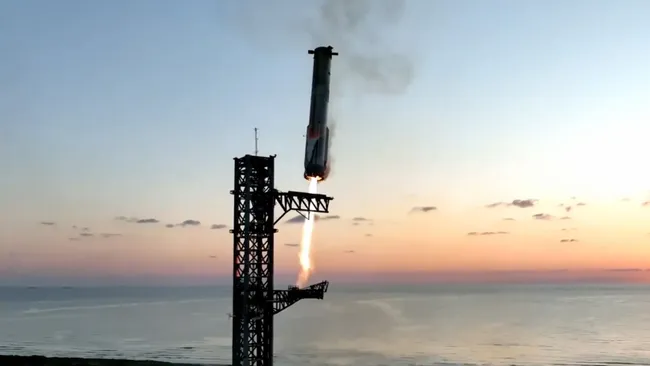
\includegraphics[width=0.95\linewidth]{figures/LiteratureStudy/StarshipCatch.jpg}
    \caption{Starship catch. Image credit: SpaceX.$^{0}$.\label{fig:starship_catch}}
\end{figure}
\footnotetext{\url{https://www.space.com/spacex-starship-super-heavy-chopsticks-catch-near-abort} (Accessed: 04-12-2024)}

To land the rocket, precision and robust control systems are required, containing sensors, actuators and control algorithms. To understand the traditional mechanisms and algorithms used, first RETALT1's Guidance, Navigation and Control (GNC) system is reviewed and applied to our problem in \autoref{sec:GNC}. The RETALT1 project was a European Union Horizon program initiative to advance the research and development into technologies needed for for vertical landing launch vehicles. Following this, the different flight phases a two stage launch vehicle covers during ascent and landing are reviewed in \autoref{sec:flight_phases} focusing on the RETALT1 description and real-World results from Space X's \textit{Starship} launch vehicle.

Finally, current high-level trajectory optimisation methods are reviewed of loss-less convex optimisation (\cite{Acikmese2007}, \cite{Acikmese2013}, \cite{Blackmore2010} and \cite{Wang2020}) and Model Predictive Control (MPC) (\cite{Wang2018}), in \autoref{sec:convex_optimisation} and \autoref{sec:MPC} respectively. Trajectory optimisation is an important part of landing as it ensures a safe and accurate landing, while minimising fuel consumption. However, traditional methods are shown to be computationally complex, which can limit their real-time application effectiveness, causing a trade-off between solution optimality and real-time feasibility. Advances in machine learning in the field of deep reinforcement learning were neural networks are used as function approximators how provided a potential solution independent of the trade-off. Deep reinforcement learning (DRL) in terms of applications to the rocket landing problem are presented in \autoref{sec:DRL}.

\subsection{Guidance, Navigation and Control architecture}
\label{sec:GNC}

RETALT1's GNC system takes in sensor readings and a reference trajectory to provide actuator commands. First the \textbf{flight manager} sets the flight phase, for example vertical rising or boostback burn. Then, the \textbf{navigation module} takes in sensor readings and adjusts them when required through techniques like filtering or state estimation to estimate the state of the rocket. With the flight phase given from the flight manager, the estimated state from the navigation model and the reference profile already generated the \textbf{guidance module} provides a reference attitude and actuation commands to the \textbf{control module}, using feedback to augment its outputs (control reference). Finally, the \textbf{control module} actuators the actuators. This process is shown clearly in \autoref{fig:GNC_architecture}.

This provides a modular architecture, which data-driven control methods could unify into a smaller framework providing a GNC system with less complexity and smoother flight phase transitions. On the other hand, data-driven methods could also replace individual blocks like Guidance and Control, acting as an end-to-end controller, or generate an optimal reference trajectory and optimise the switching conditions in the flight manager. In summary, data-driven methods could increase the performance RETALT1's GNC system in different ways.

To better understand the state of the vehicle one can have without complex state-estimation techniques, the sensors are looked at. These are listed below, and the total observable state space is created in \autoref{eq:total_obs}; this can be used with the control system design to use the observable states as feedback. Mass states are added as the mass used can be estimated through throttle commands.
\begin{itemize}
    \item Inertial Measure Unit (IMS): measures acceleration and angular velocity through gyroscopes and accelerometers.
    \item Global Navigation Satellite System (GNSS): provides the rocket's position, but on Mars is unavailable as there are no satellites in orbit there which perform GNSS requirements.
    \item Differential Global Positioning System (DGPS): is similar to GNSS, but provides more accurate position information through a ground-based correction.
    \item Flush Air Data System (FADS): measures aerodynamic parameters like dynamic pressure, static pressure, angle of attack, side-slip angle and Mach number.
    \item Altimeter: measures altitude.
\end{itemize}

\begin{equation}
    \mathbf{o} = \bigg[ \underbrace{\{x, y, z, h\}}_{\text{Position}}, \underbrace{\{\vec{v}, \vec{a}\}}_{\text{Linear states}}, \underbrace{\{q_0, q_1, q_2, q_3\}}_{\text{Quaternions}}, \underbrace{\{\omega_x, \omega_y, \omega_z\}}_{\text{Angular velocities}}, 
    \underbrace{\alpha, \theta, \gamma, \beta}_{\text{Angles}}, \underbrace{\rho, M, p_a}_{\text{Aerodynamics}}, \underbrace{m_{\text{prop}}, m}_{\text{Masses}}\bigg]
\label{eq:total_obs}
\end{equation}

To control the rocket actuators must be able to provide forces and moments in each axis. First, each thruster has a main valve to initiate or shut-down the thruster. Second, for a full-flow staged combustion cycle, where the propellants are gasified in pre-burners which are used to drive turbopumps in main combustion chamber, the turbopump's rpm is altered to throttle the engines. Throttling is needed during ascent to avoid the rocket reaching maximum dynamic pressure, likewise in landing, but along with providing precise velocity control.

To adjust the flight path of the rocket to allow it to flow a curved mission profile, torque is needed to rotate the rocket, for the thrusters the Thrust Vector Control (TVC) system performs this (\cite{sutton_rocket_2016}). A gimballed pivot TVC system is chosen for this case study, as it is a "simple, proven technology" (\cite{sutton_rocket_2016}) and used upon Space X's rockets.

However, during periods of propulsive free flight or otherwise called "\textit{ballistic arcs}" an actuator capable of attitude control without ignited thrusters is required. Two systems are used, first Aerodynamic Control Surfaces (ACS) are used in the denser atmosphere as they effectiveness is linearly dependent to dynamic pressure, and the Reaction Control System (RCS) for the upper atmosphere.

The RCS provides small $\Delta v$ and orientation corrections in the upper atmosphere, but as mainly used for rotation maneuver's it is called a attitude control system (\cite{sutton_rocket_2016}). The actuation side of RCS has most of the moment provide by cold-gas thruster pairs in each axis at the top and bottom of the rocket, where the moment arm is greatest. Due to the "pair" nature of the actuators they can provide a pure moment without forces. Reaction wheels can also be used for fine control without propellant consumption, but only thrusters are considered here as they provide a larger moment. Not that, Space X don't carry propellant for them, but instead use excess ullage gas. Ullage gas is an inert non-combustible gas, like gaseous nitrogen ($N_2$) used to pressurise propellant tanks

The ACS can take several forms, considering only dynamic actuators used in industry. Super Heavy, the first stage of Space X's launch vehicle \textit{Starship} has 4 electrically actuated grid fins (\autoref{fig:gridfins}), which contain a lattice of small aerodynamic control surfaces within the fin. Mounted at the top of the first stage there is a large moment arm allowing for heavy attitude control, secondly they provide aerodynamic drag to the vehicle. Starship, the second stage of it's namesake, uses a pair of flaps at the top of bottom to control orientation allowing Starship to perform a near-horizontal "\textit{bellyflop}" landing for maximum drag.

The \textit{bellyflop} maneuver optimises landing fuel efficiency and manages re-entry forces. After re-entering Earth's denser atmosphere, Starship will re-orientate horizontally as in \autoref{fig:bellyflop}, significantly reducing drag and terminal velocity, while distributing heating loads across the vehicles stables. At around 500 metres above ground Starship's sea-level optimised Raptor engines reignite and the rear flaps fold inward to cause a rapid flip to vertical orientation. Asides from Space X, New Glenn, Blue Origin's re-usable launcher, uses 4 adjustable fins at the top of it's upper stage for aerodynamic orientation control.

\begin{figure}[H]
    \centering
    \begin{subfigure}[t]{0.48\linewidth}
        \centering
        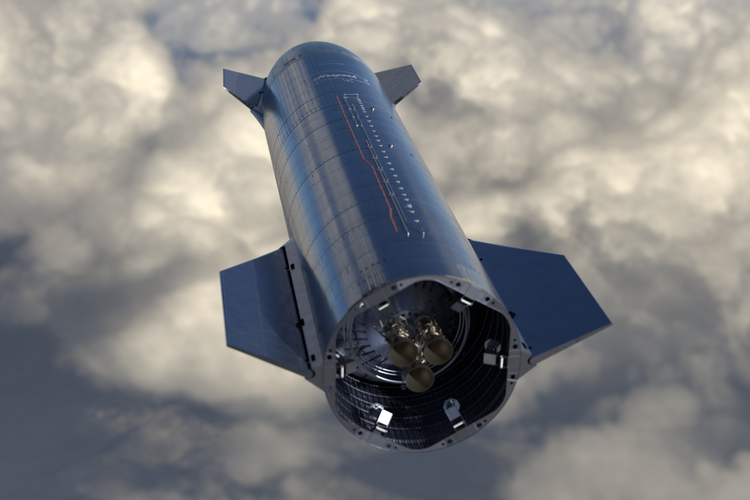
\includegraphics[width=\linewidth]{figures/LiteratureStudy/BellyFlop.png}
        \caption{Starship's orientation during bellyflop.}
        \label{fig:bellyflop}
    \end{subfigure}
    \hfill
    \begin{subfigure}[t]{0.48\linewidth}
        \centering
        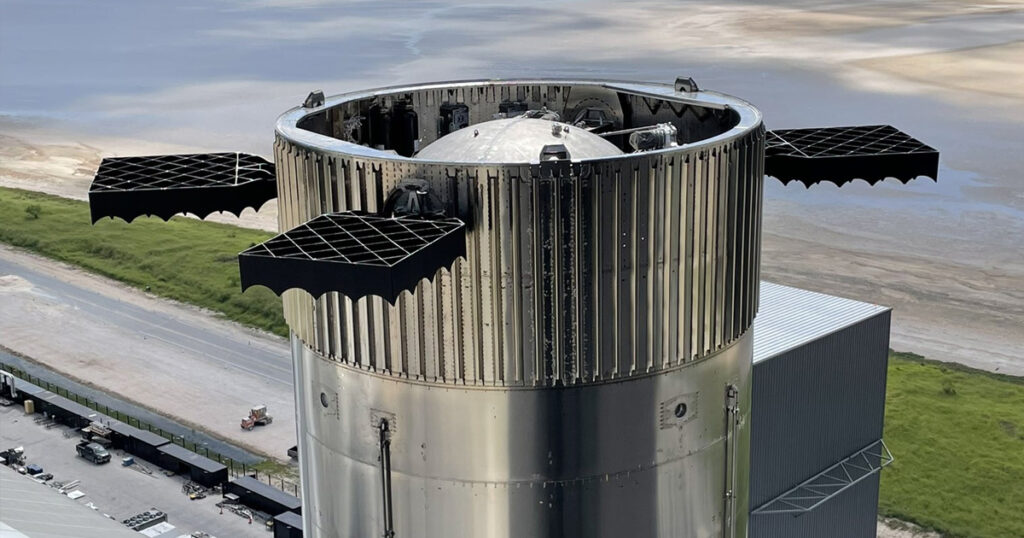
\includegraphics[width=\linewidth]{figures/LiteratureStudy/gridfin.jpg}
        \caption{Super Heavy's grid fins. (Credit: SpaceX)}
        \label{fig:gridfins}
    \end{subfigure}
    \caption{Aerodynamic control surfaces used by SpaceX vehicles.}\footnotetext{\url{https://www.thomasnet.com/insights/spacex-testing-starship-sn8-s-belly-flop-maneuver/}. Accessed on 18-05-2025.}
\end{figure}

Using Space X's Starship launch vehicle as reference, the total available action space can be constructed. This is shown below, with the RCS simplified to only a moment command.
\begin{itemize}
    \item Super Heavy contains 20 fixed perimeter engines, 13 gimballed engines, cold-gas thrusters for reaction control and four grid fins.
    \item Starship has 3 fixed vacuum optimised engines, and 3 gimballed sea-level optimised engines used for the landing burn. Also, there are pairs of fins at the top and bottom of the stage, along with a RCS.
\end{itemize}

\begin{equation}
    \mathbf{a}_{\text{superheavy}} = \bigg[\underbrace{\{\tau_i, MVM_i\}^{33}_{i=1}}_{\text{Throttle}}, 
    \underbrace{\{\theta_i^g, \psi_i^g\}^{13}_{i=1}}_{\text{Gimbal}},
    \underbrace{M_{RCS}}_{\text{RCS}}, \underbrace{\{\theta^{gf}_i, \psi^{gf}_i\}_{i=1}^{4}}_{\text{Grid Fins}}
    \bigg]
\label{eq:super_heavy_actuators}
\end{equation}

\begin{equation}
    \mathbf{a}_{\text{starship}} = 
    \bigg[
    \underbrace{\{\tau_i, MVM_i\}^{6}_{i=1}}_{\text{Throttle}},
    \underbrace{\{\theta_i^g, \psi_i^g\}^{3}_{i=1}}_{\text{Gimbal}},
    \underbrace{M_{RCS}}_{\text{RCS}}, \underbrace{\{\theta^{gf}_i\}_{i=1}^2}_{\text{Grid Fins}}\bigg]
\end{equation}

The action space can be simplified for our problem, for explain not considering roll control, removing the gimbal and grid fin angle in this direction, and reducing the number of controllable grid fins to 2. Also, for different flight phases, different actuators will be used and the others can be unconsidered, set by the flight manager along with the MVM. Finally, the gimbal and throttle commands can be uniform across each gimballed or non-gimballed thruster for a problem complexity reduction, this will reduce the time needed to learn a policy. A more complex control allocation network can be trained in further work taking into account each thruster individually.

The available action space in the reduced form for the problem is \autoref{eq:super_heavy_actuators_reduced} for the first stage and \autoref{eq:starship_actuators_reduced} for the second.

\begin{equation}
    \mathbf{a}_{\text{superheavy}} = \bigg[\tau, \theta^g, M_{RCS}, \theta^{gf}_{left}, \theta^{gf}_{right}\bigg]
\label{eq:super_heavy_actuators_reduced}
\end{equation}

\begin{equation}
    \mathbf{a}_{\text{starship}} = 
    \bigg[\tau, \theta^g, M_{RCS}, \theta^{flap}_{upper}, \theta^{flap}_{lower}\bigg]
\label{eq:starship_actuators_reduced}
\end{equation}

\begin{figure}[H]
    \centering
    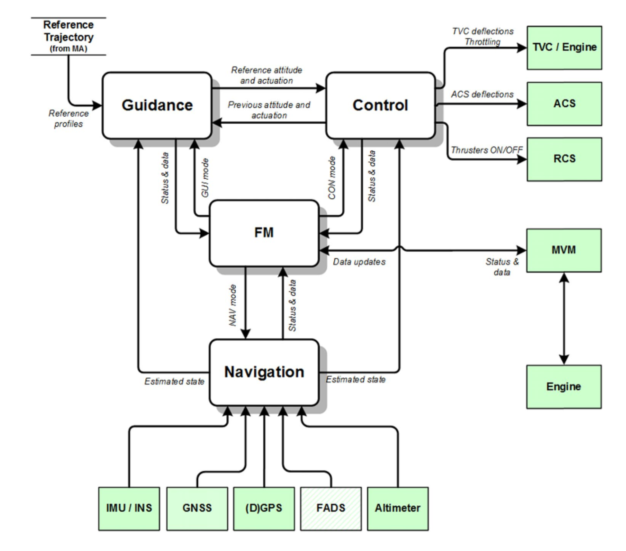
\includegraphics[width=0.95\linewidth]{figures/LiteratureStudy/GNC_architecture.png}
    \caption{RETALT1 rocket's GNC architecture for recovery (\cite{Botelho2022})}
    \label{fig:GNC_architecture}
\end{figure}

\subsection{Flight phases}
\label{sec:flight_phases}

As spoken of in the previous section, the launcher has various flight phases, these are periods of fields characterised by specific aims and atmospheric conditions.  For a two stage launch vehicle the launch starts with a \textbf{vertical rising} phase where the launcher travels vertically upwards to clear the launch tower, before the rocket performs a pitch over (\cite{Launcher_Trajectory}) called a \textbf{gravity turn} to build the horizontal velocity required for orbital insertion. The gravity turn may have to throttle the engines to avoid the launcher's maximum dynamic pressure being breached in the denser atmosphere layers. High dynamic pressure also causes greater aerodynamic forces, a low angle of attack is desired to reduce aerodynamic disturbances.

After the first stage ascent burn, stage separation will occur. In \textit{cold-staging} the fairing between the stages separate and both stages coast for a few seconds, before the second stage's engines ignite. However, Starship performs \textit{hot-staging} to ignite the second stage's engines before fairing separation. This is beneficial as it reduces gravity losses and can provide the first stage with a pitch moment to assist the flip-over manoeuvrer.

After separation, the second stage performs a burn to direct it to orbit using TVC to curve it's thrust vector and the RCS to counteract the minor angular disturbances. Following the burn, it will coast to its orbital altitude before a circularisation burn occurs. Trajectory optimisation for this "exo-atmospheric burn" may use Pontryaigin's Maximum principle to compute the thruster vector and burn time.

Meanwhile, after separation the first stage begins its landing procedure by performing a \textbf{flip over manoeuvrer} to rotate the rocket to near horizontal for a \textbf{boostback burn} to cancel the horizontal velocity. The TVC performs the flip-over manoeuvrer on a limited number of the gimballed engines, which are then fired at maximum throttle to perform the boostback burn, which cuts off the engines once a terminal horizontal velocity has been reached.

The direction of the flip over manoeuvrer depends on the landing scenario, \autoref{fig:RETALT1_flightplant} depicts these two scenarios, with scenario A showing  Return To Launch Site (RTLS) and B showing Away From Launch Site (AFLS) landings. For Space X, AFLS landings the rocket's first stage on an autonomous drone-ship downrange, and RTLS back at a landing pad near the origin launch site.

Trading off, RTLS has lower operational costs and is logistical simpler as no drone ship needs to be deployed for recover, also resulting in a faster refurbishment time as the booster is closer to the processing facilities. Secondly, there is less weather dependence as ocean conditions affect the feasibility of a AFLS landing occurring successfully. However, AFLS recovers less fuel as the boostback burn needs to remove less of the horizontal velocity and thus allows for increased payload capacity. For this scenario, RTLS will be considered do to it allowing for rapid re-usability, one of the main motivations for reusable rockets.

A \textbf{high-altitude ballistic arc} takes place after the flip over, the control authority for orientation comes from the RCS as the rocket is flying through the upper atmosphere, ACS can also assist, but in this problem is not considered.

As the rocket descends into the denser atmosphere the dynamic pressure will increase through increasing density and vertical speed. A burn then occurs to slow the rocket down to avoid dynamic pressure limits and decelerate for landing. Also, with higher dynamic pressure the ACS becomes more effective than the RCS and is used for orientation control.

For Space X's super heavy booster this burn is called the \textbf{landing burn} and the engines burn continually untill landing. However, for some mission scenairos, like RETALT1's mission profile presented in \autoref{fig:RETALT1_flightplant}, the burn is split into two burn with a \textbf{re-entry burn} to avoid the dynamic pressure limits followed by a aerodynamic phase where the ACS maneuvers the rocket, before a final \textbf{landing burn}. Space X's Super Heavy booster profile is selected as it is real-World proven.

\begin{figure}[H]
    \centering
    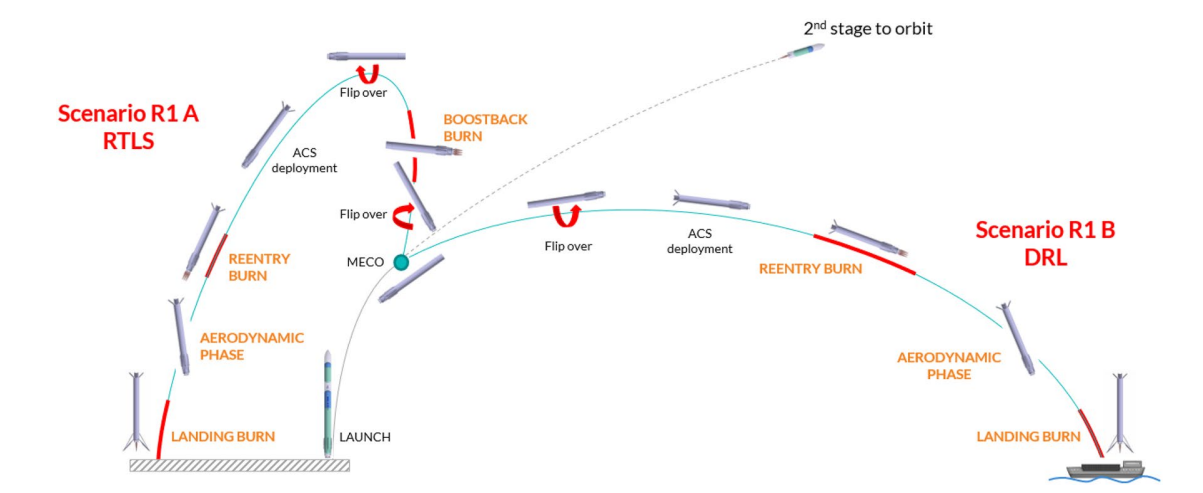
\includegraphics[width=0.95\linewidth]{figures/LiteratureStudy/RETALT1landing.png}
    \caption{RETALT1 return mission concept (\cite{dezaiacomo2022retalt})}
    \label{fig:RETALT1_flightplant}
\end{figure}

\subsection{Descent trajectory optimisation methods}
\label{sec:traj_obj_descent}

Optimal descent trajectory generation for a rocket involves balancing competing objectives leading to a multiple objective optimisation problem (MOOP). First, this MOOP aims to minimise fuel consumption while providing feasibility to the solution. Secondly, the solution must manage strict constraints throughout flight on variables like dynamic pressure and also terminal conditions at the landing site. Several optimisation frameworks have been used specifically for the rocket landing problem, each with differing solution optimality, robustness and computational requirements.

This section reviews three key approaches found in literature, first Model Predictive Control (MPC) which provides an optimal solution and updates with feedback to balance trajectory deviation and actuator usage, allowing for fuel consumption to be minimised. Secondly, the widely applied lossless convexification for rocket landing which provides reliable and efficient solutions but is computationally complex. Finally, a Deep Reinforcement Learning (DRL) approach is presented with the author's (Gaudet) argumentation as to why reinforcement learning is a valid choice.

\subsubsection{Model Predictive Control}
\label{sec:MPC}

MPC is from the optimal control family and uses constrained optimisation at each time step. Given the current state, the future states can be predicted over a finite horizon through the predicted control inputs (\cite{rawlings2017mpc}). The cost function of \autoref{eq:MPC} is minimised to determine optimal inputs, while the states and inputs can be constrained for feasibility. Here $Q$ and $R$ acts as cost weights for state deviation and control effort, setting the costs of state errors and actuation.

\begin{equation}
    J = \sum_{k=0}^{N-1} [(\mathbf{x}_{t+k} - \mathbf{x}_{\text{ref}})^T \cdot Q \cdot (\mathbf{x}_{t+k} - \mathbf{x}_{\text{ref}}) + \mathbf{u}_{t+k}^T \cdot R \cdot \mathbf{u}_{t+k}]
\label{eq:MPC}
\end{equation}

\begin{figure}[H]
    \centering
    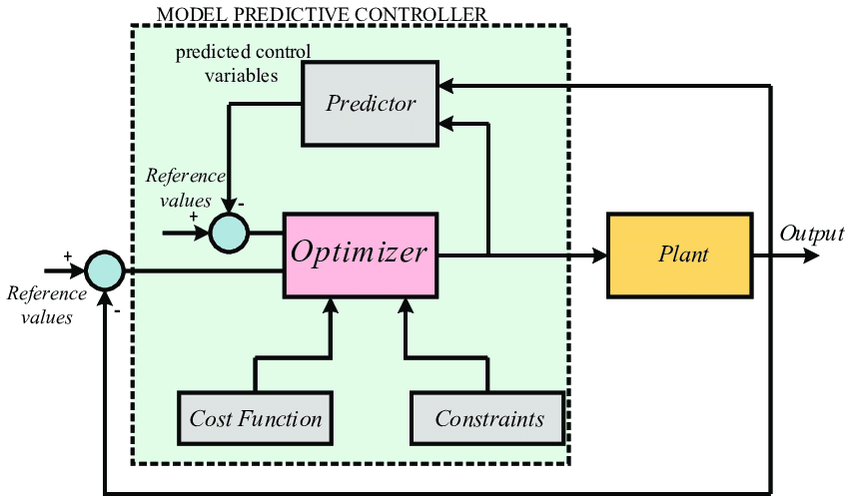
\includegraphics[width=0.95\linewidth]{figures/LiteratureStudy/MPC.png}
    \caption{A schematic of how an MPC works (\cite{Sohaib2018MPC}).}
    \label{fig:MPC}
\end{figure}

\cite{Wang2018} introduce convex-MPC for rocket landing. Stating how it solves optimisation problems while satisfying constraints. In terms of rocket landing it is constrained by dynamic pressure, landing conditions and thermal heating, and has to optimise for minimal fuel consumption. For Wang's convex MPC method the system is repeatedly linearised and non-convex constraints convexified such that convex optimiser used. Furthermore, the MPC optimises the minimisation of the usage of tracking error controls.

MPC is a nice fit for the rocket landing problem due to its ability to adapt to uncertainties in real-time as a finite-horizon optimisation problem. Secondly, it ensures optimal performance under constraints by minimising the tracking error and control effort. However, the finite-time horizon can affect it's long-term trajectory planning, leading to a trade-off between computation time and solution optimality.

\subsubsection{Lossless Convex Optimisation}
\label{sec:convex_optimisation}

% Loss-Less convexification

\cite{Acikmese2007} and \cite{Acikmese2013} use loss-less convexification on the concave rocket landing problem in the Mars environment, where the minimum thrust and thrust vector direction is convexified so that the optimal solution of the convex problem is the same as the concave problem. A lossless solution occurs when the relaxed convex problem's solution is equivalent in optimality to that of the nonconvex problems. \cite{Gaudet2018}, say that the benefit of convexification is that interior point solution methods can guarantee solutions within a bounded time.

\cite{Acikmese2007} start by describing the point mass model of their rocket; here, they assume all thrusters are identical and have the same cant angles, with the position and velocity as the decision variables. The objective is to minimise fuel consumption, which is equivalent to thrust minimisation. A simple introduction introduction of a slack variable on a nonconvex thrust constraint \(T_{\text{min}} \leq ||T(t)|| \leq T_2, \forall t \in [0, t_f]\). This allows the problem to be formulated as a Second Order Cone Programming (SOCP) problem. The constraints are convexified and formulated as a SOCP problem, then discretised into a finite-dimensional problem so optimisation solvers can handle it. This approximates the control inputs as a linear combination of basis functions.

\textit{Lemma. SOCP} (\cite{boyd2003socp})
A class of convex optimisation problems with constraints including second-order (Lorentz) cones. This is shown in \autoref{eq:SOCP}. Note that the variables used here are not in the nomenclature. f is the cost weighting, x the decision variables, m the number of constraints, and A, b, c, d, F, g constraint parameters. 

\begin{equation}
\begin{aligned}
    \text{minimise:}& f^T \cdot x \\
    \text{subject to:}& ||A_i \cdot x + b_i||_2 \leq c_i^T + d_i, i = 1, ..., m \\
    & F \cdot x = g \\
\end{aligned}
\label{eq:SOCP}
\end{equation}

\cite{Blackmore2010} focus on a minimum landing-error approach to Mars landings, aiming to minimise the final distance to the landing site when there is no feasible trajectory due to constraints. First, the algorithm assumes it is feasible and solves similar problems above; if found infeasible, a new trajectory is found to minimise landing error. \cite{Acikmese2013}, take the approaches of \cite{Acikmese2007} and \cite{Blackmore2010}, bring them together and extend them for thrust pointing constraints (cant angle). \cite{mao2017successive} introduces the Successive Convexification (SCvx) algorithm to solve this planetary landing problem with collision avoidance constraints. This algorithm iteratively convexifies the problem before using a "\textit{project-and-linearise}" procedure to transfer the non-convex constraints (state and dynamic) to convex approximations; they argue this allows for a sequence of simpler convex problems to be solved. In more detail, the current solution is iteratively projected onto the feasible set from the non-convex constraints before being linearised around the constraints. Finally, it converges in fewer iterations

% 6 Dof Quaternion problem

\cite{Szmuk_2018} extend the problem to include landing time as an optimisation problem in this 6 DoF form, using the SCvx for linearisation and discretisation into a real-time solvable SOCP problem. Furthermore, trust regions ensure the boundedness of the solution during iterations, and a virtual control avoids infeasibility from poor initial guesses. Finally, further papers with Beh\c{c}et A\c{c}\'{i}kme\c{s}e extend this algorithm with more constraints.

\cite{shen2022realtime} combine convex optimisation with deep neural networks to generate their initial guesses; this reduces computational demands to a 40.8\% reduction in computational time with 99.1\% of test cases reaching real-time requirements. This offers a proof-of-concept of the use of data-driven control techniques to imitate the optimal behaviours of a convex optimiser, albite only for the initial condition and not over the whole trajectory.

\subsubsection{Deep Reinforcement Learning}
\label{sec:DRL}

\cite{Gaudet2018} use deep reinforcement learning to solve the rocket landing problem. They argue that the need for the controller to have stability guarantees is not applicable for rocket landing, as for optimal, linear and Lyapunov (MPC) control, they can only guarantee this with an accurate and validated model, which is hard to get for a complex problem like this, they explicitly state hypersonic re-entry as the example.

Secondly, constrained policy optimisation satisfies the need for hard constraints, clipping the action so it is constrained or even modifying the reward function. Furthermore, it has the additional benefits of allowing for an integrated control (GNC) system and can compensate for sensor noise or offsets. The result was a solution to the Mars-powered descent landing problem, which was robust to parameter uncertainty and noise, on 3 and 6 DoF models.

\section{Data-driven control strategies for robust rocket landing}
\label{sec:ICS}
The rocket landing control problem is challenging, containing a high-dimensional observation and action space, along with dynamic uncertainties from the atmosphere and complex non-linear rocket dynamics, for instance, from fuel sloshing. At the same time, it needs to be safety-critical; as a result, a robust and adaptive solution must be used to compensate for the disturbances and uncertainties.

Current control methods for rocketry use loss-less convexification with SOCP solvers or an MPC to control for the trajectory which can take significant computational resources. Linear Quadratic Regulators (LQR), Proportional-Integral Derivative controllers (PID) and feed-forward models are traditional method for attitude and motion control, with proven theory allowing for stability and robustness metrics. This thesis aims to study the feasibility of using a data-driven strategy instead of currently used methods.

This is motivated by recent studies into RL applications highlighting data-driven controllers as a promising alternative to work well within the problem definition. As optimal control can be learnt through policies gained by interacting with a simulation environment without the need for complex mathematics or optimisation solvers. Secondly, they can constructed in a way to allow for robust and adaptive control. Finally, if as they are realisable they require less computational time in real-time scenairos than traditional trajectory optimisation methods.

Data-driven methods have been divided into groups focused around four main features, as presented in \autoref{fig:data_driven_family_tree}.
\begin{itemize}
    \item The learning strategy (\autoref{sec:line}) chooses whether learning will occur on of offline, determining whether they update within flight or train on a fixed dataset.
    \item Policy learning (\autoref{sec:policy}) decides to use off or on policy learning, referring whether to update the policy experiences generated by the current policy.
    \item The control has the option to use a model to guide decision making through model-based methods. Alternatively, model-free methods learn a policy through learn policies through environment interaction without use a learnt model to change its policy. \autoref{sec:model_methods} covers this.
    \item The algorithm family (\autoref{sec:TD_MC_DP_ES}) causes the best data-driven learning algorithm for the study.
\end{itemize}

\begin{figure}[H]
    \centering
    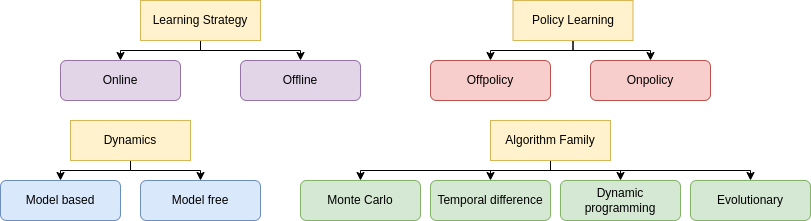
\includegraphics[width=0.85\linewidth]{figures/LiteratureStudy/DataDriven_familytree.png}
    \caption{Data driven methods family tree}
    \label{fig:data_driven_family_tree}
\end{figure}


\subsection{Online vs Offline learning}
\label{sec:line}

Policy learning can be divided into online and offline learning (\cite{sutton1998reinforcement}). Offline learning uses pre-collected data/simulations to train policies, while online learning can dynamically adapt to the environment in real time.

Offline learning allows for training before deployment, which is practical in safety-critical applications like rocket landings. As rocket landings are expensive and highly risky, it is important to learn extensively in a simulation beforehand. Online learning would allow a rocket to adapt during flight to disturbances and dynamic environments arising from the atmosphere and the complex non-linear dynamics of rocketry. However, it can lead to unpredictability and an increased computational overhead.

\textbf{Online learning}, within simulations, is chosen as the policy the rocket initially has will not be sufficient for landing. Resulting, in an updating policy needed to unlock new a better experiences bringing to a feasible landing before optimisation can occur.

\subsection{Off-policy vs On-policy methods}
\label{sec:policy}

The off/on policy decision determines how agents use their environment transitions to learn optimal policies (\cite{sutton1998reinforcement}). On-policy algorithms determine and improve the current policy executed by the agent, for instance, in SARSA, where the action-value function is updated by the agent for each action taken. Off-policy methods learn the optimal policy independently from the current actions taken during exploration; for instance, Q-learning updates the action-value function through the expected maximum cumulative rewards of future actions.

\textbf{Off-policy} methods are more sample efficient as they can reuse previous transitions through a buffer and as such is chosen. Also, in a stochastic environment, the policy updated takes into account transitions from other episodes which had different disturbances.

\subsection{Model-free vs Model-based methods}
\label{sec:model_methods}

\textbf{Model-free} control methods are well-suited for a rocket landing control system as they learn optimal policies without relying on a high-fidelity mathematical model of the dynamics and disturbances. High-fidelity models require an accurate knowledge of the non-linear and complex dynamics, which is infeasible to make by one person. Secondly, model-free methods can allow environmental exploration to adapt to uncertainties and disturbances, making them robust and adaptive. If the model-free algorithm can transfer well to higher-fidelity models, it shows a proof of concept for using data-driven control for rocket landing. Furthermore, \cite{Jiang2024} used an RL framework with "random annealing jump start" to jump-start learning and improved success rates through a model-free algorithm. Offering an indication of the initial feasibility of this project.

\subsection{Algorithm families}
\label{sec:TD_MC_DP_ES}

The rocket landing control problem has a continuous, high-dimensional state, observation and action spaces, and complex, uncertain, non-linear dynamics. \textbf{Temporal Difference} (TD), like Q-learning and State-Action-Reward-State-Action (SARSA), uses incremental learning to update value estimates from differences in actual and predicted rewards (\cite{sutton1998reinforcement}). Combining with neural networks to act as function approximators, it can effectively handle complex and continuous problems (\cite{mnih2013playing}) while being model-free.

In contrast, Dynamic Programming (DP) need full knowledge of the environment; while extensions to the method can leverage neural networks for this, it is often impractical for large systems due to the high computation requirements (\cite{cmu2021recitation}). Monte Carlo methods (\cite{sutton1998reinforcement}) average returns over complete episodes, making them less efficient for tasks like rocket landing, where long episodes may occur. Evolutionary methods optimise policies without using gradients and are parallelisable; however, they can be sample-inefficient due to a large number of policies being ran to cover the search space. As such, TD methods are chosen as they seem the most relevant to the problem.

\section{Reinforcement Learning}
\label{sec:RL}
Reinforcement learning (RL) is a topic in machine learning where \textit{agents} are trained to learn decisions through environment interaction, as visualised in \autoref{fig:RL_model}. A \textit{reward function} indicates the solution's optimality, leading the agent to converge to an optimal policy, where the actions that maximise reward are known for each state. For the problem of robust and optimal rocket landing control, RL presents a promising solution to handling the dynamic and uncertain atmosphere environment and managing high-dimensional control tasks. Unlike traditional model-based methods, deep reinforcement learning uses a neural network as a function approximator to create a model-free control, if done right, with the ability to adapt to uncertainties and unseen scenarios.

\begin{figure}[H]
    \centering
    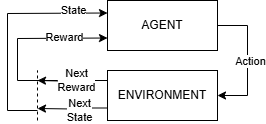
\includegraphics[width=0.65\linewidth]{figures/LiteratureStudy/RL_diagram_basic.png}
    \caption{Reinforcement Learning Model}
    \label{fig:RL_model}
\end{figure}

The aim of the section is to explain the theory behind methods of model-free, off-policy and online learning RL methods, and to survey techniques which can be used to help stabilise and speed up learning, before evaluating the best choice to move forward with. First, the foundations to give the reader a foundation in DRL, Q-learning is explained in \autoref{sec:Q_learning}. Then types of replay buffers are documented in \autoref{sec:buffers} to allow for off-policy learning. As exploration is key to unlocking new control strategies for the agent, a literature review of exploration strategies relevant for this problem is done in \autoref{sec:exploration}. Following this, the algorithms used for learning a problem of our specification are provided in \autoref{sec:off_policy}. Types of mathematical normalisation functions are analysed in \autoref{sec:normalisation_functions} to aide the stability and efficiency of training. Finally, the initial algorithm options are selected in \autoref{sec:RL_algo_selection}.

\subsection{Q-learning}
\label{sec:Q_learning}
A value-based algorithm with an agent learning values of action-state pairs to choose the resulting actions to maximise rewards, \cite{watkins1992q}. This is an off-policy algorithm, so it learns the optimal policy independent of the agent's actions, allowing for model-free RL, as the agent learns the optimal action-value function \(Q^*(s, a)\) through interacting with the environment, providing the maximum expected rewards \(R(s_t, a_t)\) from acting \(a_t\) in the state \(s_t\). The function is updated through \autoref{eq:Qlearning}, where the parameters of the Q-network are updated periodically to equal those of the target network. Here, the discount $\gamma$ determines the importance of future rewards, and $\tau$ affects how quickly new information is learnt.


\begin{equation}
    Q(s_t, a_t; \theta) \leftarrow Q(s_t, a_t; \theta) + \tau [ R(s_t, a_t) + \gamma \max_{a_{t+1}} Q(s_{t+1}, a_{t+1}; \theta^{-}) - Q(s_t, a_t; \theta)]
\label{eq:Qlearning}
\end{equation}

This section then discusses the extension of the Q-learning algorithm in the form of Deep Q-learning (DQN), which leverages neural networks acting as function approximators to apply Q-learning to high-dimensional problems. Duelling Q-networks can help in scenarios with sparse rewards, and double Q-learning is shown to help reduce value function overestimation bias.

\subsubsection{Deep Q-learning}
\label{sec:DQN}

DQN was developed to learn how to play Atari 2600 games best, \cite{mnih2015human} and \cite{mnih2013playing}. DQN allows learning of more complex environments, overcoming Q-learning's "curse of dimensionality" through generalisation over similar states. The Q-learning rule of \autoref{eq:Qlearning} takes weights \(\theta\) approximated from a neural network. In contrast, the neural network's weights are updated through a Mean-Squared Error (MSE) loss function alike \autoref{eq:DQNloss}. Secondly, target networks are again used to periodically update the parameters of the online network every set number of steps, reducing oscillations and producing a more stable loss.

\begin{equation}
    L(\theta) = \mathbb{E} [ ( R(s_t, a_t) + \gamma \max_{a_{t+1}} Q(s_{t+1}, a_{t+1}; \theta^{-}) - Q(s_t, a_t; \theta) )^2]
\label{eq:DQNloss}
\end{equation}

\subsubsection{Dueling Q-networks}
\label{sec:Dueling}

When learning, certain actions gain no rewards even though they are beneficial. For instance, when playing football, if you were to score a goal, you get a point; however, no points are gained for tackling the opposition or providing an excellent cross into the box, although they want to be encouraged. To encourage this type of behaviour in places where actions have less effect on the outcome, a duelling network architecture is proposed in \cite{wang2016dueling}. In this network, the state value and action advantage are separated into a value stream \(V(s)\) showing the state value and an advantage stream \(A(s,a)\) giving the advantage of the action. As a result, the Q-Network update rule is changed to \autoref{eq:DuelingQnetworks}.

\begin{equation}
    Q(s, a; \theta, \theta^{A}, \theta^{V}) = V(s; \theta, \theta^{V}) + \left( A(s_t, a_t; \theta, \theta^{A}) - \frac{1}{|\mathcal{A}|} \sum_{a_{t+1}} A(s_t, a_{t+1}; \theta, \theta^{A}) \right)
\label{eq:DuelingQnetworks}
\end{equation}

\begin{figure}
    \centering
    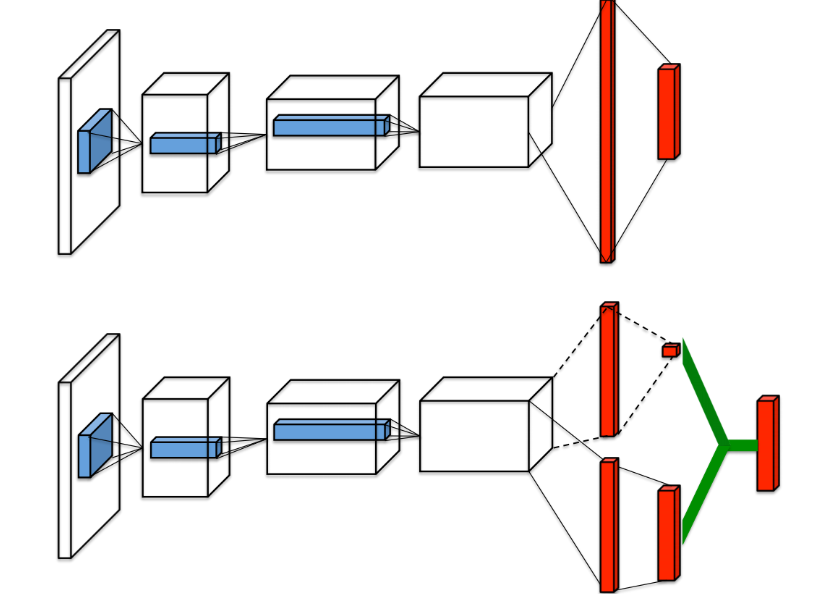
\includegraphics[width=0.5\linewidth]{figures/LiteratureStudy/RL_diagram_Dueling.png}
    \caption{\cite{wang2016dueling}. The top network is a standard Q-network, and the bottom network has a duelling architecture with two separate streams, the value and advantage streams.}
    \label{fig:enter-label}
\end{figure}

\subsubsection{Double Q-learning}
\label{sec:Double_Q_learning}

Standard DQNs tend to be biased towards over-optimistic value estimations due to the same Q-network selecting and evaluating the action. As a result, van Hasselt \cite{vanhasselt2016deep} proposed decoupling the selection and evaluation stages through a \textit{Double Q-network}, this showed to give better estimates and performances in complex environments.

These two Q-networks use the update rule of \autoref{eq:DoubleQLearning} where the leading network, parameters \(\theta\), is updated each iteration for action \(a_{t+1}\) selection, while the target network, parameters \(\theta^{-}\) evaluates these actions. After a set interval, the target network is updated to lower the over-estimation bias.

\begin{equation}
    Q(s_t, a_t; \theta) \leftarrow Q(s_t, a_t; \theta) + \alpha \left[ R(s_t, a_t) + \gamma Q(s_{t+1}, \arg\max_{a_{t+1}} Q(s_{t+1}, a_{t+1}; \theta); \theta^{-}) - Q(s_t, a_t; \theta) \right]
\label{eq:DoubleQLearning}
\end{equation}

\subsection{Replay buffers}
\label{sec:buffers}
Off-policy methods have increased sample efficiency through their ability to reuse experiences from previous transitions. For an environment like rocket landing where the manoeuvrer can take minutes leads to an episode with 1000s of steps when discretised by a modest 0.1s time step. Allowing the data to reused provides the agent with a broader range of experiences to update from is exploration is present. The \textit{replay buffer} holds the transition data such that they can be reused later on.

The first instance of the replay buffer was the \textbf{uniform replay buffer} used to play Atari games, \cite{mnih2013playing}, here transitions are stored in a First-In-First-Out manner with all samples having equal probability of being sampled to provide diverse training samples. The buffer stores the state, action, reward and next state for random batches of experiences to be sampled during training; this breaks the correlations of consecutive episodes.

\textbf{Prioritised Experience Replay} (PER) was then introduced to take actions with a better learning potential through sampling via their temporal difference (TD) error, \cite{schaul2015prioritized}. TD measures the prediction and target networks' Q-value differences, as shown in \autoref{eq:TD_error}. The immediate reward is summed with the future rewards (when active) and subtracted from the current Q-value estimate. A small constant is added to get the priority, with 'i' being the transition; this computes the probability $P(i)$. The hyperparameter $\tilde{\alpha}$ sets the importance of sampling previous transitions with a higher reward probability. The weights \(w_i\) are updated through \textit{importance sampling} where the hyperparameter $\tilde{\beta}$ determines the correction; trading off between faster learning and bias correction. 

\begin{equation}
\begin{aligned}
    e_{TD} =& |R(s_t, a_t) + (1 - \text{done}) \cdot \gamma \cdot \max_{a_{t+1}} Q(s_{t+1}, a_{t+1}; \theta^-) - Q(s_t, a_t; \theta)| \\
    \Tilde{p}_i =& e_{TD,i} + 10^{-5} \\
    P(i) =& \frac{p_i^{\alpha_{\text{PER}}}}{\sum_k p_k^{\alpha_{\text{PER}}}} \\
    w_i =& \left( \frac{1}{N \cdot P(i)} \right)^{\beta_{\text{PER}}}
\label{eq:TD_error}
\end{aligned}
\end{equation}

\textbf{Hindsight Experience Replay} (HER) is a goal-orientated replay buffer where an episode is replayed with a different goal the agent was trying to achieve. This replay buffer enhances learning efficiency for environments with sparse or delayed rewards. HER takes the states from failed episodes as alternative goals to generate valuable strategies for successful experiences. For example, if a robotic arm places an object in a different position, HER can leverage this as a new goal, leveraging failed trajectories to create additional data and improve sample efficiency. The algorithm to implement HER is shown in \cite{andrychowicz2017hindsight}.

\subsection{Exploration strategies}
\label{sec:exploration}

Exploration strategies balance the sensitive exploration and exploitation trade-off. Exploration is needed, especially in the early stages of learning a new part of the episode, to allow the agent to uncover new experiences which maximum the Q-value. Meanwhile, exploitation is also needed to force the agent to converge through taking the path with the maximum Q-value at that point.

Exploration strategies can be divided into two use cases: discrete spaces, $\epsilon$-greedy (\cite{sutton1998reinforcement}) and Boltzmann, and continuous spaces. For rocket landing, the state space (e.g., position, velocity, orientation) and the action space (e.g., thrust levels, gimbal angles) are continuous; as such only these strategies continuous strategies are covered.

\textbf{Action noise-based exploration} is an efficient way to encourage exploration in continuous space by adding noise.
\begin{itemize}
    \item \textit{Gaussian Noise}: in \cite{lillicrap2015continuous}, the exploration policy is created by adding random noise to the actor's policy. This is used in several actor-critic RL configurations used for learning on a continuous domain, like the Twin Delayed Deep Deterministic Policy Gradient (TD3) algorithm wrote in \autoref{sec:TD3}.

    \item \textit{Ornstein-Uhlenbeck (OU) noise}: is used to temporary correlate noise, \cite{lillicrap2015continuous} use this to enhance their exploration efficiency, showing it is good for "physical control problems with inertia".

    \item \textit{Adaptive Noise Scaling}: can be combined with a method above to balance exploration-exploitation during training. Here the noise is scaled is automatically altered, like in soft actor critic (SAC) shown in \autoref{sec:SAC}
\end{itemize}

\begin{tcolorbox}[title={\textbf{Lemma. Gaussian and OU noise}}]
Exploration in deterministic reinforcement learning methods like DDPG, D4PG or TD3 explained later in \autoref{sec:off_policy} requires the injection of external noise into the policy's action space to discover new and unseen solutions.  Two common types of noise processes are Gaussian and OU noise.

\textbf{Gaussian noise} is temporally uncorrelated and drawn independently at each timestep from a normal distribution. This noise is simple and suitable for environments where smoothness in action evolution over time is not critical.
\[
    \epsilon_t \sim \mathcal{N}(0, \sigma^2)
\]


\textbf{Ornstein–Uhlenbeck noise} introduces temporal correlation by modelling the stochasticity as mean-reverting process, meaning that the stochastic process tends to revert towards a long term mean. This mean-reverting proces temporally smooths noise, idea for physical control tasks with momentum like rocket landing where a sudden change in action can lead to instability. The correlation across timesteps simulates inertia, yielding more natural and consistent exploration trajectories.

\[
    \epsilon_{t+1} = \epsilon_t + \theta (\mu - \epsilon_t) \Delta t + \sigma \sqrt{\Delta t} \mathcal{N}(0, 1)
\]

Gaussian noise is simpler to implement than OU noise, however OU noise encourages smoother transitions in systems with momentum, like physical control tasks.
\end{tcolorbox}


\textbf{Parameter Space Noise} (PSN) was introduced to overcome the downfall of the action space noise of inconsistent exploratory behaviours due to a fixed state always giving different actions. This can give problems like early truncation where at points in the episode the action is sensitive to noise and needs to be precise. However, adaptive noise scaling to push the action space noise to small amounts at parts in the episode can overcome this problem. PSN adds noise through \autoref{eq:PSM} to perturb the policy network parameters at the start of each episode and maintain them fixed afterwards; this results in state-dependent actions, unlike Gaussian noise methods.

\begin{equation}
    \tilde{\theta} = \theta + \mathcal{N}(0, \sigma^2 \cdot I)
\label{eq:PSM}
\end{equation}

PSN has been experimented with in \cite{plappert2018parameter}, building on the work of \cite{sehnke2010parameter} and \cite{rucksties2008state}; they show PSN offers better exploration and avoids suboptimal converge on continuous environments, and has significant benefits in environments with sparse rewards, along with outperforming Evolutionary Strategies (ES).


In environments where extrinsic rewards are sparse, intrinsic rewards can allow the agent to explore better; this can be employed through an \textbf{Intrinsic Curiosity Module} (ICM) developed in \cite{pathak2017curiosity}, which encourages the agent to explore. Intrinsic rewards are provided by the agent's own experience, motivating them to explore without extrinsic rewards.

An inverse model, which predicts the action \(\hat{a}(s_t, s_{t+1})\), is trained via \autoref{eq:loss_ICM_inverse} to minimise the loss between the actual and predicted actions. The forward model predicts the next state's features \(\hat{\phi}_{s_{t+1}}(\phi_{s_t}, a_t)\), through minimisation in state feature prediction via \autoref{eq:loss_ICM_forward}. The intrinsic reward, \autoref{eq:intrinisic_reward}, depends on the hyperparameter $\eta$ acting as the scaling factor. The total resulting reward is the sum of the extrinsic and intrinsic rewards.

\begin{equation}
    L_I(\hat{a}_t, a_t; \theta^I) = -\log P(a_t | s_t, s_{t+1}; \theta^I)
\label{eq:loss_ICM_inverse}
\end{equation}

\begin{equation}
    L_F(\phi(s_t), \hat{\phi}(s_{t+1}; \theta^F)) = \frac{1}{2} \|\phi(s_{t+1}) - \hat{\phi}(s_{t+1}; \theta^F)\|^2
\label{eq:loss_ICM_forward}
\end{equation}

\begin{equation}
    R^{\text{intrinsic}}_t = \eta \cdot \frac{1}{2} \|\phi(s_{t+1}) - \hat{\phi}(s_{t+1}; \theta^F)\|^2
\label{eq:intrinisic_reward}
\end{equation}

An alternative to ICM is \textbf{Random Network Distillation} (RND), introduced in \cite{burda2018exploration}, where they argue it is simpler and more stable than ICM, through testing on Montezuma's Revenge. This method works well for sparse reward environments, allowing extrinsic and intrinsic rewards to be flexibly combined. Here, intrinsic rewards are based upon a prediction error from a trainable "prediction" network approximating a fixed and randomly initialised "target" network. The prediction network is trained to minimise the prediction error through \autoref{eq:RND_1}. The intrinsic reward can be set equal to the prediction network loss, as such states explored less will gain a higher prediction error, and thus, the RND encourages them to be explored; this process is visualised in \autoref{fig:RND}. In essence, RND measures how novel a state is by comparing prediction error on a fixed random target network.

\begin{equation}
    L_{\text{predict}} = \frac{1}{2} \cdot ||y_{\text{target}} - y_{\text{predict}} ||^2 = r_{\text{intrinsic}}
\label{eq:RND_1}
\end{equation}

\begin{figure}[H]
    \centering
    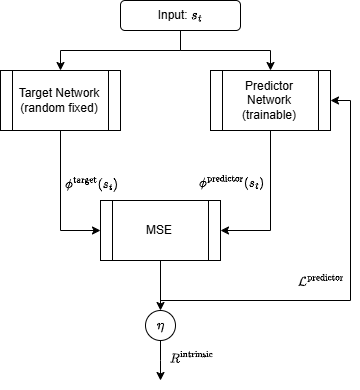
\includegraphics[width=0.5\linewidth]{figures/LiteratureStudy/RL_diagram_RND.png}
    \caption{Flow diagram showing how RND works.}
    \label{fig:RND}
\end{figure}

\textbf{Noisy networks} (\cite{fortunato2017noisy}) incorporate parametric noise into the network weights to enhance exploration efficiency via stochastic diversity of the agent's policy. Here, Stochastic Gradient Descent (SGD) learns the noise scale, adapting it over time; for instance, less noise is present as the agent becomes more confident, decreasing exploration. The authors also show how it is compatible with any RL architecture which employs SGD. Ultimately arguing, noisy networks provide structured and adaptive exploration.

\subsection{Off-Policy Continuous On-Line Methods}
\label{sec:off_policy}
As reasoned in \autoref{sec:ICS} an online offpolicy method which works with a continuous action and observation space is the chosen method due to its sample efficiency. The actor-critic framework is the commonly used to learn an optimal policy for online and continuous domain problems. The actor learns the optimal policy by Q-value maximisation; maximising the expected cumulative return from taking a given action in a given state. So the actor, \(\zeta(s_t; \theta^Z)\), learns the action for each state to maximise expected return through \autoref{eq:maxQ_AC}, with the mapping of state to action learnt through a neural network acting as a function approximator. The critic estimates the state-action value \(Q(s_t, a_t; \theta^Q)\); the expected reward for taking an action in a given state, this is used by the actor to update its policy. The critic is used instead of raw rewards to train the actor because it reduces the variance of policy gradient updates by providing smoothed action-value estimates.

Meanwhile, the critic learns to minimise TD error \footnote{Defined in \autoref{sec:exploration}.}. For example, \autoref{eq:TD_AC} shows the scenairo for a critic where the TD error between the predicted state-action pair and the critic's target network.

\begin{equation}
    \mathcal{L}_Q(\theta^Q) = \frac{1}{N_{\text{buffer}}} \cdot \sum_{i=1}^{N_{\text{buffer}}}(R^i(s^i_t, a^i_t) + \gamma \cdot Q'(s^i_{t+1}, \zeta'(s^i_{t+1};\theta^{\zeta'});\theta^{Q'}) - Q(s^i_t, a^i_t; \theta^Q))^2
\label{eq:TD_AC}
\end{equation}

\begin{equation}
    \mathcal{L}_\zeta(\theta^\zeta) = - \frac{1}{N_\text{buffer}} \cdot \sum_{i=1}^{N_{\text{buffer}}} Q(s^i_t, \zeta(s^i_t;\theta^\zeta);\theta^Q)
\label{eq:maxQ_AC}
\end{equation}

The following subsections cover 5 of the main continuous online offpolicy reinforcement  learning algorithms found in literature. SAC and Maximum a posteriori Policy Optimisation (MPO) learn a stochastic policy, while Deep Deterministic Policy Gradient (DDPG), Distributed Distributional Deterministic Policy Gradient (D4PG) and TD3 learn a deterministic policy.

\subsubsection{Deep Deterministic Policy Gradient method}
\label{sec:DDPG}

DQNs work with a discrete action space, as such with a continuous control problem the continuous outputs have to be discretised leading to massive a massive action dimension, inhibiting learning. DDPG was presented by \cite{lillicrap2015continuous} to be a solution to this problem through an extension to the Deterministic Policy Gradient (DPG) method (\cite{silver2014deterministic}), allowing for a model-free offpolicy online actor-critic algorithm with neural networks utilised as deep function approximators to learn a policy and state-action value function in continuous domains.

The actor provides deterministic actions with the critic approximating the resulting Q-value. \cite{mnih2015human} utilise target networks and experience replay, like in DQNs, to stabilise training and improve sample efficiency, and OU noise is used for action noise-based exploration like explained in \autoref{sec:exploration}.

To summarise DDPG is an actor-critic framework with extensions being:
\begin{enumerate}
    \item Action-space-based noise used for exploration.
    \item Target networks used to improve learning stability, through Polyak averaging \autoref{eq:target_networks}.
\begin{equation}
\begin{aligned}
    \theta^{Q'} \leftarrow& \tilde{\tau} \cdot \theta^Q + (1 - \tilde{\tau}) \cdot \theta^{Q'}\\
    \theta^{\zeta'} \leftarrow& \tilde{\tau} \cdot \theta^\zeta + (1 - \tilde{\tau}) \cdot \theta^{\zeta'}
\end{aligned}
\label{eq:target_networks}
\end{equation}
    \item A replay buffer \(\mathcal{R}\) for off-policy learning, improving sample efficiency.
\end{enumerate}

\begin{tcolorbox}[title={\textbf{Lemma. Target network updates via Polyak averaging}}]
In deep reinforcement learning tasks target networks are often used to stabilise learning by slowly the changing of targets used for value estimation. Instead of directly copying the online netwrok's weights, they are soft updated through \textit{Polyak averaging}..

employed to stabilise learning by providing slowly changing targets for value estimation. Instead of directly copying the online network's weights to the target network, a soft update method called \textit{Polyak averaging} is used.

Let \( \theta \) denote the parameters of the online network and \( \theta^{'}\) the parameters of the corresponding target network. The Polyak update rule is defined as:
\[
    \theta^{'} \leftarrow \tau \theta + (1 - \tau) \theta^{'} 
\]
where \( \tau \in (0, 1) \) is the averaging coefficient, a larger coefficient tracks the target network faster and can induce instability. Alternatively, a small coefficient gives stable but slower updates which can enhance robustness.

Polyak averaging ensures the parameters of the target network move slowly towards that of the online network, reducing oscillations and divergence in value estimation, to promote learning stability.
\end{tcolorbox}

\subsubsection{Distributed Distributional Deterministic Policy Gradients}
\label{sec:D4PG}

\cite{barthmaron2018d4pg} extended DDPG to D4PG to include a distributional critic promotes learning stability, along with PER for faster learning and N-step returns for improving the rewards over longer-time horizons.
\begin{itemize}
    \item A distributed framework is used, where multiple actors asynchronously generate experiences and fill a shared replay buffer, where a central learner updates the policy.
    \item A \textit{distributional critic} is used, essentially instead of modelling a scalar \(Q(s,a; \theta^Q)\) it predicts a probability distribution \(Q_Z(s,a; \theta^{Q_Z})\) over all possible returns, this distribution modelling works well for stochastic environments where differing Q values can come from different actions in the same state. The critic now outputs a probability distribution leading to KL divergence used instead of MSE for the loss function.
    \item N-steps are used to give the reward over a longer time horizon, this is beneficial for task where there are long-term dependencies, such as in rocket landing. The N-step reward equation is shown in \autoref{eq:N_step_rewards}.
\end{itemize}

\begin{equation}
    y^i_t = \bigg(\sum_{m=0}^{N_{\text{episode}}} \gamma^m \cdot R(a^i_m, s^i_m)\bigg) + \gamma^{N_{\text{episode}}} \cdot Q_Z'(s^i_{N_{\text{episode}}}, \zeta'(s^i_{N_{\text{episode}}}; \theta^{\zeta'}); \theta^{Q'})
\label{eq:N_step_rewards}
\end{equation}

\begin{tcolorbox}[title={\textbf{Lemma. N-step returns}}]
In traditional TD learning the value estimate of a state is updated based on the immediate reward and the estimated discounted value of the next state. \autoref{eq:one_step_rewards} is the equation for calculated the 1-step return at time t ($G_t^{(1)}$ ) using the immediate reward ($R_{t+1}$) and the estimated value of the next state ($V(s_{t+1})$).

% $G_t^{(1)}$ is the 1-step return at time t
% $R_{t+1}$ is the immediate reward
% $\gamma$ is the discount factor
% $V(S_{t+1})$ is the estimated value of the next state

\begin{equation}
    G_t^{(1)} = R_{t+1} + \gamma V(s_{t+1})
\label{eq:one_step_rewards}
\end{equation}

N-step returns extends this concept to look ahead $n$ steps through \textit{booststrapping} the fine value estimate.ping. \autoref{eq:n_step_rewards} shows the generic formula for n-step rewards. N-step returns allows the agent to learn from a longer sequence of rewards before bootstrapping, giving it more information about long-term dependencies

\begin{equation}
    G_t^{(n)} = R_{t+1} + \gamma R_{t+2} + \gamma^2 R_{t+3} + ... + \gamma^{n-1} R_{t+n} + \gamma^n V(S_{t+n})
\label{eq:n_step_rewards}
\end{equation}

This formula changes when terminal states are within the trajectory length set for n-step returns ($n$), otherwise called within the n-step horizon. The returns should only include rewards up to the terminal state, either a truncated or completed episode, with no bootstrapping or rewards after termination. If step $t+k$ is a terminal state,where $k < n$), the n-step return becomes \autoref{eq:n_step_rewards_terminal}.

\begin{equation}
    G_t^{(n)} = R_{t+1} + \gamma R_{t+2} + ... + \gamma^{k-1} R_{t+k}
\label{eq:n_step_rewards_terminal}
\end{equation}
\end{tcolorbox}

\subsubsection{Twin Delayed DDPG}
\label{sec:TD3}


\cite{fujimoto2018addressing} use double Q-learning in an actor-critic format to reduce overestimation bias of the value function through a pair of independent critics and double Q-learning. Through their approach, they run DDPG with two extensions:
\begin{enumerate}
    \item Clipped Gaussian noise is used instead of OU for action space-based noise; clipped noise is chosen to prevent sharp action value changes causing over-fitting.
    \item Through the use of double Q-learning (dual critics), the loss functions for the critic have the "target critic changed" to the minimum between the networks, ensuring the most conservative estimate. For the actor loss, only the primary Q-network is considered; this ensures it is based on a single Q-value estimate reducing noise and learning instability.
\end{enumerate}

\subsubsection{Soft Actor-Critic}
\label{sec:SAC}

\cite{haarnoja2018soft} introduce SAC as an actor-critic algorithm which maximises both expected rewards and the policy's entropy, encouraging exploration and thus leading to more robust policies. 
TD3 uses Gaussian action space noise, whereas SAC's actor outputs a Gaussian distribution \(\zeta_S(s;\theta^{\tilde{\zeta}}, \theta^\mu, \theta^\sigma)\), with the subscript "S" denoting it as a stochastic actor. This actor outputs \(\mu(s_t; \theta^\mu)\) and \(\sigma(s_t; \theta^\mu)\), which are converted to a noisy action through \autoref{eq:SAC_actor}. Compared to TD3, the difference is that the noise distribution is a learned parameter providing \textit{state-dependent exploration}.

\begin{equation}
\begin{aligned}
    \sigma(s; \theta^\mu) = e^{\log \sigma(s; \theta^\mu)} ,\quad
    \tilde{a} = \mu(s; \theta^\mu) + \sigma(s; \theta^\mu) \odot \epsilon ,\quad
    \epsilon \sim \mathcal{N}(0,I) ,\quad
    a = tanh(\tilde{a})
\end{aligned}
\label{eq:SAC_actor}
\end{equation}

\begin{figure}[H]
    \centering
    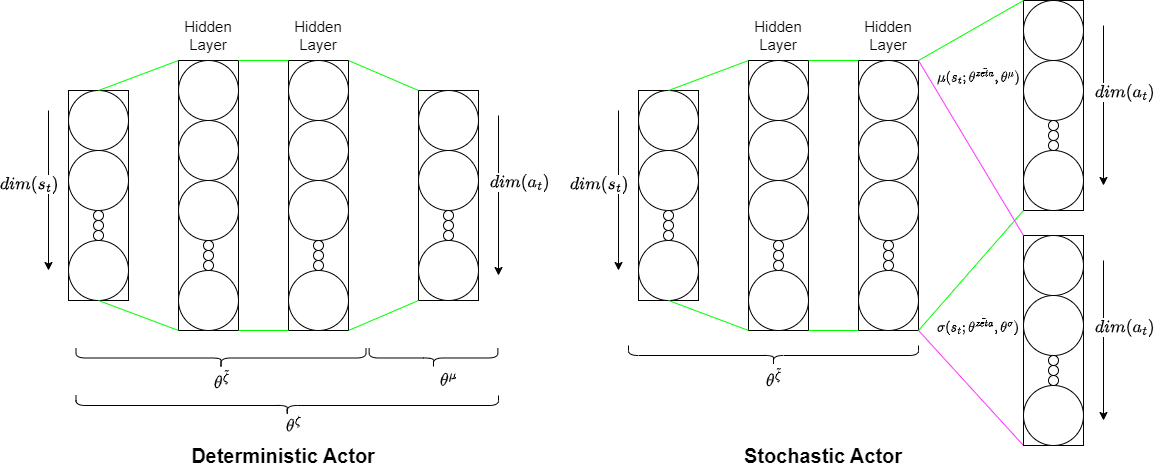
\includegraphics[width=0.95\linewidth]{figures/LiteratureStudy/RL_diagram_ActorNetworks.png}
    \caption{Diagram showing the differences in actor networks, for deterministic and stochastic.}
    \label{fig:actor_networks}
\end{figure}

SAC has an additional entropy term to control the state-dependent exploration. \textit{Temperature} $v$ updates to encourage an entropy to meet the target entropy controlling the degree of randomness and traditionally set as  \(\mathcal{H}_{\text{target}} := -\dim(a_t)\). \autoref{eq:SAC_temperature} temperature is updated to encourage the negative Gaussian likelihood equal to the target entropy.

\begin{equation}
    \mathcal{L}_{\log(\nu)} = \frac{1}{N} \cdot \sum_{i=1}^{N}-\log(\nu) \cdot \bigg(\log p(a_t^i|\mu,\sigma^2)+\mathcal{H}_{\text{target}}\bigg)
\label{eq:SAC_temperature}
\end{equation}


\begin{tcolorbox}[title={\textbf{Lemma. Gaussian likelihood}}]
The Gaussian likelihood is the probability density function of a normal distribution evaluated at a given point. For a random variable \( x \in \mathbb{R}^d \), with mean \( \mu \in \mathbb{R}^d \) and standard deviation \( \sigma \in \mathbb{R}^d \), the log-likelihood is given by:
\[
\log p(x \mid \mu, \sigma^2) = -\frac{1}{2} \left[ \frac{(x - \mu)^2}{\sigma^2} + 2 \log \sigma + \log(2\pi) \right]
\]
The Gaussian likelihood shows how likely point $x$ is under the $\mu$ and $\sigma^2$. The first term is called the \textit{quadratic term} and penalises deviations from the mean scaled by the variance. The second term called the \textit{normalisation term} accounts for the distribution spread, and the final term is a constant ensuring proper normalisation.

A lower negative log probability, \textit{Gaussian likelihood}, indicates the sample is more likely under the distribution, while a high negative log probability indicates a less likely sample under the distribution.
\end{tcolorbox}

The actor has two terms in its loss function, first an entropy regularisation term, where the log probability gives a metric for the likelihood of the actor, weighted by the temperature. The temperature updates previously to balance entropy through changing the entropy regularisation loss magnitude in the reward function. The second term extracts the minimum of two q network outputs, alike double q-learning, to reduce overestimation bias; this term encourages the policy to select the actions of that state with the highest expected returns.

\begin{equation}
    \mathcal{L}_{\zeta^S} = \frac{1}{N} \cdot \sum^N_{i=1} \bigg(\nu \cdot \log p(a_t^i|\mu, \sigma^2) - \min_{i=1,2}Q(s_t^i,a_t^i;\theta^{Q_i})\bigg)
\label{eq:SAC_actorloss}
\end{equation}

The TD error is computed to represent the mean-squared Bellman error for each critic, which is trained to minimised the square difference between its predicted Q-value and the shared TD target, through the loss function of \autoref{eq:SAC_critic_loss}.

\begin{equation}
\begin{aligned}
    TD_{\text{target}} =& R_t + \gamma \cdot (1-d) \cdot \bigg(\min_{i=1,2} \{Q'(s',a';\theta^{Q'})\}- \nu \cdot \log p(a'|\mu',(\sigma')^2)\bigg) \\
    e_{TD} =& \frac{1}{2} \cdot \bigg((TD_{\text{target}} - Q_1)^2 + (TD_{\text{target}} - Q_2)^2\bigg)
\end{aligned}
\label{eq:TD_error_entropy_regularised}
\end{equation}

\begin{equation}
    \mathcal{L}_Q = \frac{1}{N} \cdot \sum^N e_{TD}
\label{eq:SAC_critic_loss}
\end{equation}

% SAC in a distributed format
SAC has been used to perform many tasks, \cite{wahid2020learning} used it in a distributed form to perform control and navigation tasks. While \cite{akimov2019distributed} used it in a distributed framework to update a shared replay buffer and used a multivariate reward representation to have sub-rewards allowing for transfer learning, which utilises knowledge distillation to increase learning speed.

% STOPPED HERE
\subsubsection{Maximum a posteriori Policy Optimisation}
\label{sec:MPO}

\cite{schulman2015trpo} introduced Trust Region Policy Optimisation (TRPO) as an iterative procedure for policy optimisation suitable to large non-linear policies of neural networks. Here a trust region controls the update between policies through Kullback-Leibler (KL) divergence. \cite{schulman2017proximal} presented Proximal Policy Optimisation (PPO) as a first-order approximation of the second-order optimisation TRPO. The paper states have PPO is simler, more generic and of better sample efficiency than TRPO, and consistently outperforms other onpolicy online methods like Advantage Actor-Critic (A2C).

PPO is a stochastic actor-critic framework which prevents large updates causing instability through constraints on the deviation of the policy through their KL divergence.

\begin{tcolorbox}[title={\textbf{Lemma. KL divergence}}]
The KL divergence is a measure of how one probability distribution \( P \) diverges from a second, reference distribution \( Q \). For continuous distributions with probability densities \( p(x) \) and \( q(x) \), the KL divergence from \( Q \) to \( P \) is defined as:
\[
\mathcal{D}_{\mathrm{KL}}(P \parallel Q) = \int p(x) \log \frac{p(x)}{q(x)} \, dx
\]
The smaller the KL divergence the more identical the distributions are.
\end{tcolorbox}

PPO was first employed without a value function, where the advantage estimate \(\hat{A}_t\) is equal to the Monte Carlo return \(G_t(s_t, a_t) = \sum_{k=0}^\infty \gamma^k \cdot R_{t+k}(s_t, a_t) \). From here, a clipped surrogate objective is used to update the policy, as shown through the second equation in \autoref{eq:PPO}. Note that the other objectives, including a KL divergence-based penalty, were used and showed decreased performance.

\begin{equation}
\begin{aligned}
    \text{No clipping or penalty:}& \mathcal{L}(\theta) = r_t(\theta) \cdot \hat{A}_t(s_t, a_t) \\
    \text{Clipped:}& \mathcal{L}(\theta) = \min\{r_t(\theta)\cdot\hat{A}_t(s_t, a_t), \text{clip}(r_t(\theta), 1 - \epsilon^{\text{PPO}}, 1 + \epsilon^{\text{PPO}}) \cdot \hat{A}_t(s_t, a_t) \\
    \text{KL penalty:}& \mathcal{L}(\theta) = r_t(\theta) \cdot \hat{A}_t(s_t, a_t) - \beta^{\text{PPO}} \cdot \text{KL}[\zeta_{\text{old}}(s_t; \theta^{\zeta_{\text{old}}}) || \zeta(s_t; \theta^\zeta)] \\
    \text{With:}& r_t(\theta) = \frac{\zeta(s_t; \theta^\zeta)}{\zeta_{\text{old}}(s_t; \theta^{\zeta_{\text{old}}})}
\end{aligned}
\label{eq:PPO}
\end{equation}

The actor-critic PPO was introduced to improve sample efficiency via value function estimation to stabilise the advantage function estimate by \autoref{eq:PPO_critic}. Here, the critic is trained to minimise the value loss through MSE \(MSE[G_t, V_t]\).

\begin{equation}
\begin{aligned}
    G_t(s_t, a_t) =& \sum_{k=0}^\infty \gamma^k \cdot R_{t+k}(s_t, a_t) \\
    A_t(s_t, a_t) =& G_t(s_t, a_t) - V(s_t; \theta^\zeta) \\
\end{aligned}
\label{eq:PPO_critic}
\end{equation}

%MPO
\cite{abdolmaleki2018maximum} introduce MPO as an off-policy version to PPO, which has better sample efficiency. They state it boasts the robustness, insensitivity to hyperparameter changes, and scalability of an on-policy algorithm while having the off-policy sample efficiency due to their utilisation of a replay buffer. MPO decouples PPO into two steps:
\begin{enumerate}
    \item Optimisation of a non-parametric target policy.
    \begin{itemize}
        \item The intermediate policy with a probabilistic representation of the value function.
        \item \(\nu\) controls the steepness of distribution, in essence controlling the exploration-exploitation trade-off.
        \item It doesn't rely on a neural network and is computed for the value function, acting like a "soft target" or a reference policy.
    \end{itemize}
    \item Parametric policy updating for target approximation.
    \begin{itemize}
        \item The actual policy which the agent uses to interact with the environment, parametrised through a neural network.
        \item Updates through minimisation of the KL divergence with its non-parametric policy.
    \end{itemize}
\end{enumerate}

The target policy is updated through \autoref{eq:Estep} called the \textit{E-Step} (expectation step). Note that the actor is stochastic, like SAC.

\begin{equation}
    \zeta_{\text{S, target}}(s_t; \theta^{\zeta_{\text{target}}}) \varpropto  \exp\left(\frac{Q(s, a)}{\nu}\right)
\label{eq:Estep}
\end{equation}

The parametric policy is updated through minimisation of the KL divergence of the target and parametric network, as shown in \autoref{eq:PPO}, incorporating  KL divergence constraint to stay within the trust region. Meanwhile, the critic is updated as normal.

The temperature parameter is updated through dual optimisation of \autoref{eq:MPO_dual}, here \(\epsilon^\nu\) controls the variance of the weights for regularisation. \cite{prior2024jaxrl}, use Sequential Least Squares Programming (SLSQP) is used to minimise the dual function concerning $\nu$, with a softmax function used to normalise the new weights, \autoref{eq:MPO_softmax}.


\begin{equation}
    g(\eta) = \nu \cdot \epsilon^{\nu} + \eta \cdot [\mathbb{E}_{s\sim R}[\log(\frac{1}{N_{\text{buffer}}}\cdot\sum_{i=1}^{N_{\text{buffer}}}\exp(\frac{Q(s, a_i; \theta^Q)}{\nu^*}))]]
\label{eq:MPO_dual}
\end{equation}

\begin{equation}
    w_i = \frac{\exp(\frac{Q(s, a_i)}{\eta})}{\sum_j \exp(\frac{Q(s, a_j)}{\eta})}
\label{eq:MPO_softmax}
\end{equation}

The actor updates through the log-likelihood of the target and current policies, as is a multi-variate Gaussian distribution. Secondly, it has two Lagrangian multipliers \(\lambda^\mu\) and \(\lambda^\sigma\) to maintain the constraints on the KL divergence between the target and current policy's Gaussian distributions. Pre-defined thresholds \(M^\mu\) and \(M^\sigma\) define the \textit{trust region}. This process is shown in \autoref{eq:MPO_actor}.

\begin{equation}
\begin{aligned}
    \mathcal{L}^\sigma &= \lambda^\sigma \cdot \left(M^\sigma - D_{KL}(\zeta^{\text{target}}(s_t; \theta^\sigma) \parallel \zeta(s_t; \theta^\sigma))\right), \\
    \mathcal{L}^\mu &= \lambda^\mu \cdot \left(M^\mu - D_{KL}(\zeta^{\text{target}}(s_t; \theta^\mu) \parallel \zeta(s_t; \theta^\mu))\right), \\
    \mathcal{L}^{\zeta, \text{unconstrained}} &= - \frac{1}{N^{\text{buffer}}} \sum_{i=1}^{N^{\text{buffer}}} \Big( \log P(a_i \mid \mu^{\text{target}}(s_t; \theta^\mu), \sigma(s_t; \theta^\sigma)) \\
    &\quad + \log P(a_i \mid \mu(s_t; \theta^\mu), \sigma^{\text{target}}(s_t; \theta^{\sigma^{\text{target}}})) \Big).
\end{aligned}
\label{eq:MPO_actor}
\end{equation}


The \textit{"Maximum a Posteriori"} framework balances the exploration-exploitation trade-off through a trust region. Like SAC, a temperature parameter \(\nu\) controls the system's entropy. The authors tested it on control tasks \textit{Walker-2D}, \textit{Acrobat}, and \textit{Hopper}; it was shown to outperform DDPG and PPO in an extensive ablation study. However, there is limited evidence of whether it can outperform more advanced DDPG algorithms like D4PG, SAC or TD3.

\cite{prior2024jaxrl} implement this scheme in JAX (\cite{jax2018github}) with a double critic alike TD3. Deduced to be used to reduce overestimation bias; secondly, they clip the gradient of the loss function for the actor update. Finally, target networks are used.

The original paper runs the MPO algorithm in a distributed form, with a single learner but multiple learners (agents) collecting data independently, with a \text{chief} collecting the gradients and performing a parameter update through averaging gradients. In other words, \textit{distributed synchronous SGD}.


Finally, MPO can be used in a distributed framework, with the user able to configure it however they like. \cite{hoffman2020acme} implemented DMPO in their Acme framework, using distributional critics similar to D4PG.

\subsection{Normalisation functions}
\label{sec:normalisation_functions}
Normalisation can be applied to observations, actions and rewards to stabilise training and brining values within the same range. ADD MORE MOTIVATION. In this section different types of normalisation shall be presented.

$\mathbf{\tanh}$ \textbf{normalisation:} smooths saturation of large values to squish outliers between $(-1,1)$. The $k$ factor can be selected to give the maximum expected value equal to an output of say 0.8, such that there is room for outliers beyond on that.

\begin{equation}
    x' = \tanh(k \cdot x)
\end{equation}

\textbf{Min-max normalisation:} is a simple linear scaling, which is interpretable, but is sensitive to outliers.

\begin{equation}
    x' = \frac{x - \min(x)}{\min(x) - \max(x)}
\end{equation}

\textbf{Shifted normalisation:} zero centers the data but does not reduce it to within a range.

\begin{equation}
    x' = x - \mu(x)
\end{equation}

\textbf{Exponential scaling:} amplifies large value while suppresses small values to increase contrast. This can be useful for some scenarios where reward shaping wants large values to be emphasized.

\begin{equation}
    x' = e^{k \cdot x}
\end{equation}

\textbf{Logarithmic scaling:} is used to compress large values and expand small ones to reduce the dynamic range. It is useful to stabilise large-magnitude inputs, providing an alternative to $\tanh$ and clipping. Also, it can be bounded to between 0 and 1 through its denominator.

\begin{equation}
    x' = \frac{\log(1 + x)}{\log(1 + \max(x))}
\end{equation}

\subsection{Reinforcement learning algorithm selection}
\label{sec:RL_algo_selection}
The reinforcement learning section of the literature study has covered key concepts in online offpolicy reinforcement learning algorithms. In terms of learning for a physical control task, the rocket will need state-dependent exploration to ensure no sudden changes in action and at times a lower noise when the action is sensitive. For instance when travelling near the dynamic pressure limit of the rocket the grid fin angles will be more sensitive to a change in state than for at lower angles. Furthermore, the injected noise should scale with the magnitude of the mean action, since for example the physical effect of a deviation from a small gimbal angle is less significant than the same deviation at larger angles.

OU noise performs better than Gaussian noise to prevent sudden changes as is a mean-reverting process. However, MPO and SAC have a trainable stochastic network allowing for state-dependent exploration. As such, MPO and SAC are the two chosen algorithms. ICM and RND at intrinisic rewards to the network, which is beneficial in sparse environments, but if the reward function during landing is set to increase extrinisic rewards it diminishes the need for these and reduces the number of learnable parameters. Noisy networks and PSN provide exploration through injecting noise into the weights of the network, this will only be trialled if the exploration from the selected RL algorithm is insufficient.

% Buffer
As an offpolicy methods requires the ability to reuse experiences from previous transitions, these must be stored in a buffer. \autoref{sec:buffers} covers three types of buffer, first the simple uniform replay buffer to randomly sample transitions, then the PER which focuses on action with better learning potential, and finally HER a goal-orientated buffer enhancing learning efficiency for environments with sparse or delayed rewards. As set previously, the reward function will be non-sparse, giving HER to have limited benefit. The implementation of PER can be based on a uniform buffer's code skeleton, so the algorithm can have the option to set both a uniform and prioritised replay buffer.

% N-step rewards
In D4PG Barth-Maron use N-step rewards to change the value estimate from using only immediate reward and the estimated value of the next step to n-step returns. Here the reward is propagated over multiple steps before bootstrapping the value network. A richer and temporally extended learning signal is provided, which will benefit the rocket in working with delayed rewards through enhancement of credit assignment over the trajectory.

In the context of a landing rocket, this scenairo could be avoiding maximum dynamic pressure, as the maximum dynamic pressure a rocket reaches is dependent on the previous actions taken of the whole trajectory rather than the only the final action before the limit is reached. Also, for it allows for the terminal reward to be propagated throughout the trajectory.

The trade-off is that N-step returns other a more informative reward to promote learning efficiency but increase the variance of the rewards, as such it is important to scale the reward assigned through \autoref{eq:n-step-scaling-factor} to take into account n-step propagation. The trajectory length chosen must be long enough to propagate the rewards, but if it is too long it will increase variance. A trajectory length which is too long can be discovered through a high variance on sampled rewards from the buffer or a large kurtosis, along with the critic struggling to reduce TD errors.

\begin{equation}
    R_t = R_t \cdot \frac{1-\gamma}{1-\gamma^n}
\label{eq:n-step-scaling-factor}
\end{equation}

The trade-off is that N-step methods may increase variance, but this is typically offset by improved learning efficiency when combined with experience replay. The use of off-policy algorithms like SAC and MPO makes this compatible with replay buffers, allowing for stable N-step learning from past transitions.

\begin{tcolorbox}[title={\textbf{Lemma. N-step reward scaling factor}}]
To ensure consistency in the magnitude of returns between 1-step and n-step temporal difference updates, the n-step rewards must be scaled appropriately. Consider the case where the per-step reward \( R \) is constant. The n-step return becomes:
\[
G_t^{(n)} = \sum_{k=0}^{n-1} \gamma^k R = R \cdot \sum_{k=0}^{n-1} \gamma^k
\]
This is a finite geometric series and evaluates to:
\[
G_t^{(n)} = R \cdot \frac{1 - \gamma^n}{1 - \gamma}
\]
To match the scale of a 1-step reward, the reward at each step can be rescaled by the inverse of the geometric sum:
\[
R_t^{\text{scaled}} = R_t \cdot \frac{1 - \gamma}{1 - \gamma^n}
\]
This correction ensures the total magnitude of accumulated rewards remains consistent across different choices of \( n \), reducing instability from overly large return targets in long-horizon settings.
\end{tcolorbox}

% L2 regularisation
Regularisation is technique used in machine learning to reduce a networks overfitting and encourage its ability to generalise. In terms of a critic this can cause the critic to overfit to reduce a few outlying large TD errors reducing its generalisability to the rest of the data. As for the actor, it can generalise well for specific states, but struggles in new unseen scenairos. To regularise the critic L2 regularisation (\cite{krogh1992weightdecay}), otherwise known as weight decay, shall be used to discourage large weights.

\begin{tcolorbox}[title={\textbf{Lemma. L2 regularisation (weight decay)}}]
L2 regularisation improves the generalisation of neural networks by penalising large weight magnitudes, through a quadratic penalty term added to the loss function, modifying the loss to:

\[
\mathcal{L}_{\text{total}} = \mathcal{L}_{\text{original}} + \lambda \lVert \theta \rVert_2^2
\]
where \( \lambda \) is a L2 regularisation coefficient hyperparameter controller the strength of the regularisation. This penalty encourages the optimiser to find small-weight solutions; which become less sensitive to noise and decrease likelihood of overfitting. Empirical evidence from Krogh and Hertz (1992) supports the effectiveness of L2 regularisation in improving generalisation across a wide range of tasks.
\end{tcolorbox}

\cite{andrychowicz2020matters} investigated the impact of different normalisation techniques, a form of regularisation. First they showed how input normalisation benefits most RL environments. For an environment like rocket landing were altitude can vary tens of thousands of meters and pitch angle to a few degrees, input normalisation is required. As the critic takes in both action and observation, both need to be normalised. To bound the states, they will be normalised between -1 and 1 through selected normalisation functions per state, by \autoref{sec:normalisation_functions}. The actor's network outputs will be bounded a $\tanh$ activation function to ensure the mean is $\in (-1,1)$ which can then be scaled to the resulting action, through functions of the inverse of \autoref{sec:normalisation_functions}.

They also review gradient clipping, although they note it of secondary importance, they show it does benefit learning stability. Here the magnitude of gradients of backpropagation are bounded 
to provide a safety net against exploding gradients, needed in high-variance environments, which could occur with the use of n-step rewards. Finally, reward normalisation will take place to reduce the variance of rewards and ensure no drastic changes in reward throughout the episode.

\begin{tcolorbox}[title={\textbf{Lemma. Gradient clipping (global norm scaling)}}]
Gradient clipping regularises training through prevention of gradient explosion to stabilise it through bounding the update step. The global L2 norm of all gradients across the network is computed:
\[
\lVert g \rVert = \sqrt{ \sum_i \sum_j g_{ij}^2 }
\]
If this norm exceeds a user-defined threshold \( \tau \), all gradients are scaled uniformly by a factor:
\[
\text{scale} = \min\left(1, \frac{\tau}{\lVert g \rVert + \varepsilon} \right)
\]
where \( \varepsilon \) is a small constant added for numerical stability. Each parameter's gradient \( g_i \) is then rescaled:
\[
g_i \leftarrow g_i \cdot \text{scale}
\]
\end{tcolorbox}

% MPO vs. SAC

\section{Rocket model}
\label{sec:RocketModel}

To learn a policy for optimal landing an \textit{environment} is needed in the form of a rocket model. As this study provides aims to provide a benchmark for determining the feasibility of using policy learning to provide control to a rocket during landing, and no proprietary model is available, a new model is constructed based of physics and literature. First, to ensure a feasible landing the rocket is sized and staged through reviewing a case study rocket from industry in \autoref{sec:SpaceX} and then a paper which optimal stages a reusable rocket in \autoref{sec:OptimalStaging}. Following this an aerodynamic model is derived with parameters found from literature in \autoref{sec:Aerodynamics}, before the same with the grid fins acting as the manoeuvrable aerodynamic control surfaces in \autoref{sec:ACS}. Following this, the atmosphere and thruster models are found and derived in \autoref{sec:Atmosphere} and \autoref{sec:RocketEngines} respectively. Finally, the model is culminated into its equations of motion in \autoref{sec:EoM}.


\subsection{Starship case study}
\label{sec:SpaceX}

To ensure the rocket has the ability to land, it must be sized to be feasible. Currently their are only a handful of proven rockets with the ability to vertically takeoff and land, these are from \textit{Space X} and \textit{Blue Origin}. To size reasonable parameters for the rocket, the \textit{Starship} launch vehicle from Space X shall be reviewed, this is a two stage launcher with the first stage called the \textit{Super Heavy Booster}, and a second stage called its namesake \textit{Starship}. The mass of each stage is shown in \autoref{tab:starship_parameters}, with their structural coefficients calculated through \autoref{eq:structural_coeff}. This launcher is able to carry 100-150 tonnes to LEO orbit, and 27 to GEO orbit (\cite{SpaceX2020_StarshipGuide}).

\begin{equation}
    \epsilon = \frac{m_s}{m_s + m_p}
\label{eq:structural_coeff}
\end{equation}

\begin{table}[htbp]
    \centering
    \caption{Mass and performance parameters of \textit{Super Heavy} and \textit{Starship}}
    \label{tab:starship_parameters}
    \begin{tabular}{@{}lcc@{}}
        \toprule
        & \textbf{Super Heavy booster} & \textbf{Starship} \\ \midrule
        Total mass [t]                          & 3,675 & 1,600 (excluding payload) \\
        Propellant mass [t]                     & 3,400 & 1,500 \\
        Structural mass [t]  & 275    & 100 \\
        Structural coefficient [-] & 0.0748 & 0.0625 \\ \bottomrule
    \end{tabular}
\end{table}

In terms of propellant, both stages use a fuel oxidiser mixture of liquid oxygen ($LOX$) and liquid methane ($LCH_4$) called methalox. The 2nd stage carries 1170 kg of $LOX$ and 330 kg $LCH_4$, giving a oxidiser-fuel ratio of 3.545; this is taken to be the same for the first stage too due to the same engines, Raptor 3, being used.


The Raptor 3 engines are top of the range full-flow cycle engines, with two varieties. One optimised for sea-level performance which is used on the 1st stage. The second is optimised for vacuum performance, with the 2nd stage taking 3 of these for ascent and 3 sea-level optimised engines for descent. From the specific impulse, a measure of rocket efficiency giving the thrust produced per unit flow of propellant, the exhaust velocities are calculated through \autoref{eq:exhaust_velocities}. As the engines are optimised for sea-level and vacuum, the nozzle exit pressures are assumed to be close to the pressure in those regimes to minimise the pressure losses, \autoref{eq:pressure_losses}. The parameters of the Raptor 3 engine variants are displayed in \autoref{tab:raptor3}.

\begin{equation}
    v_{ex} = I_{sp} \cdot g_0
\label{eq:exhaust_velocities}
\end{equation}

\begin{equation}
    T_{\text{pressure losses}} = (p_e - p_a) \cdot A_e
\label{eq:pressure_losses}
\end{equation}

\begin{table}[h!]
    \centering
    \caption{Parameters of the Raptor 3 engines}
    \label{tab:raptor3}
    \begin{tabular}{@{}lcc@{}}
        \toprule
        & \textbf{Sea-level Raptor 3 } & \textbf{Vacuum Raptor 3} \\ \midrule
        Specific impulse [s] & 350 & 380 \\
        Exit diameter [m] & 1.3 & 1.3 \\
        Exit area [$m^2$] & 1.327 & 2.3 \\
        Thrust [$MN$] & 2.745 & 2 \\
        Engine mass (integrated) [kg] & 1525 (1720) & 1525 (1720) \\
        Exhaust velocities [$m/s$] & 3433.5 & 3727.8 \\
        Exit pressure estimate [$kPa$] & 101 & 0 \\
        Engine Height [$m$] & 3.1 & 4.6 \\
        \bottomrule
    \end{tabular}
\end{table}


The thrust-to-weight ratio ($TWR$) is a crucial parameter affecting how much acceleration the rocket can produce, especially at take-off. The engines produce a certain thrust, resulting in the $TWR$ determining how many engines are on the rocket. The $TWR$ is calculated through \autoref{eq:TWR} to give the stage's $TWR$ in \autoref{tab:TWR}.

\begin{equation}
    TWR = \frac{T^e_i \cdot n^e_i}{m_i \cdot g_0}
\label{eq:TWR}
\end{equation}

\begin{table}[h!]
    \centering
    \caption{Stage's thrust-to-weight ratio.}
    \label{tab:TWR}
    \begin{tabular}{@{}lcc@{}}
        \toprule
        & \textbf{Super Heavy booster} & \textbf{Starship} \\ \midrule
        Number of engines [-] & 33 & 6 \\
        Stage Thrust-to-Weight ratio [-] & 2.51 & 0.7645 \\
        \bottomrule
    \end{tabular}
\end{table}

Space X's $TWR$ can be used to decide the number of engines on a different sized rockets. The TWR for each stage can be used to calculate the stage's maximum thrust, mass flow and number of engines from its initial mass by \autoref{eq:n_e}.


\begin{equation}
\begin{aligned}
    T^{req}_i =&  m_i(0) \cdot g_0 \cdot TWR_i\\
    n^e_i =& [\frac{T^{req}_i}{T^{engine}_i}] \\
    T^{max}_i =& n^e_i \cdot T^{engine}_i \\
    \dot{m}_i^{max} =& \frac{T^{max}_i}{v_{ex}^i}
\end{aligned}
\label{eq:n_e}
\end{equation}



%Resultingrocketwidthandgiballledetccc
\subsubsection{Number of engines}
The number of engines is used to size the width of the rocket, such that the rocket can fit the required number of engines. \autoref{fig:Raptor_Comparison} shows the layout of the Raptor engines for the Super Heavy Booster, they layour with 20 fixed engines in the outer ring, followed by an inner ring of 10 gimballed engines and a central triangle of gimballed engines, totalling in 20 fixed engines and 13 gimballed engines. Taking the three centrally gimballed engines as fixed independent of the rocket's configuration, the number of engines within the ring are altered, knowing that 2 extra outer ring engines are needed to fit one extra gimballed engines.

\begin{equation}
    r_r = r_{\text{superheavy}} \cdot (1 + \frac{n_{\text{outer}} - n_{\text{outer,superheavy}}}{n_{\text{outer,superheavy}}})
\end{equation}

\begin{figure}[H]
    \centering
    \begin{subcaptionbox}{Raptor 3 engine\footnotemark[1]\label{fig:Raptor_3}}[0.35\linewidth]
        {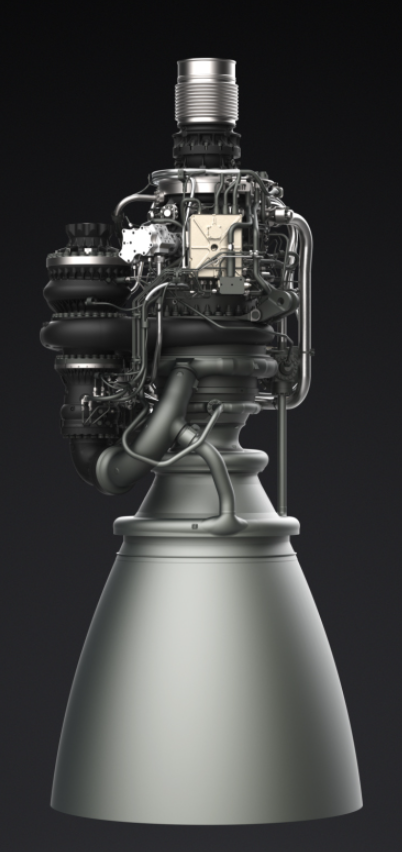
\includegraphics[width=\linewidth]{figures/LiteratureStudy/raptor_3.png}}
    \end{subcaptionbox}
    \hfill
    \begin{subcaptionbox}{Super Heavy engines\footnotemark[2]\label{fig:SuperHeavyEngines}}[0.58\linewidth]
        {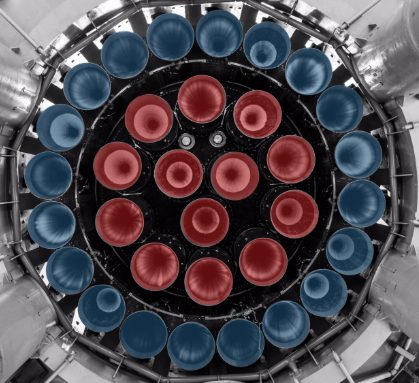
\includegraphics[width=\linewidth]{figures/LiteratureStudy/SuperHeavyRaptorLayour.png}}
    \end{subcaptionbox}
    \caption{Raptor 3 and Super Heavy engine layout}
    \label{fig:Raptor_Comparison}
    \footnotetext[1]{\url{https://www.spacex.com/vehicles/starship/}}
    \footnotetext[2]{\url{https://everydayastronaut.com/spacex-raptor-engine-comparison/}}
\end{figure}

\subsection{Optimal staging of a reusable rocket}
\label{sec:OptimalStaging}
As said in the previous section, a rocket must be sized such that it is feasible to land. If the Space X size was to be used it may not be feasible within in our model due to lower fidelity aerodynamics, or incorrect reporting of values from Space X. This results in a rocket needing to be independently sized. The method of \cite{ReusbaleStaging} is followed to size a two stage rocket with an reusable first stage and an expendable second stage.

First \autoref{eq:descent_eps} uses the first stage's structural coefficient for descent to calculate the velocity increment to descend. The structural coefficient for first stage descent is unknown, but can be the paper's value can be used. Later, this parameter can be updated from a trajectory optimiser results.

\begin{equation}
    \Delta v_{d,1} = v_{ex,1} \cdot \ln(\frac{1}{\epsilon_{d,1}}) \rightarrow \epsilon_{d,1} = e^{-\frac{\Delta v_{d,1}}{v_{ex,1}}}
\label{eq:descent_eps}
\end{equation}

The optimal staging procedure, as like expendable rockets, sets a parameter (here $\kappa$) in the X of the Tsiolkovsky equation, for \cite{ReusbaleStaging} this becomes \autoref{eq:Lagrangian_Tsiolkovsky}. When this equation is solved for $\kappa$ then the payload ratio shall be minimised, in turn minimising take off mass. The velocity increment required is found from the desired semi-major axis, \autoref{eq:v_req}.

The optimal staging procedure is similar to that of an expendable rocket. It starts by introducing a Lagrange multiplier $\kappa$ to perform constrained optimisation of the Tsiolkovsky rocket equation. This yields \autoref{eq:Lagrangian_Tsiolkovsky}, which when solved produces $\kappa$ to maximise the payload ratio; the fraction of the rocket's take-off mass consisting of payload. To do this the velocity increment required is set from the orbital velocity at the defined semi-major axis, as shown in \autoref{eq:v_req}.

To ensure feasibility of the Lagrange multiplier $\kappa$ the following constraints are added to ensure physical and mathematical validity:

\begin{itemize}
    \item \textbf{Exhaust velocity bound:} ensures $\kappa$ avoids singularities in the logarithmic expression.
    \[
    0 < \kappa < \min(v_{ex,1}, v_{ex,2})
    \]
    \item \textbf{Logarithm argument positivity:} guarantees that the logarithm's values are strictly positive to prevent undefined values.
    \[
    \frac{v_{ex,i} - \kappa}{v_{ex,i} \cdot \epsilon_i} > 0 \quad \Rightarrow \quad \kappa < v_{ex,i}
    \]
\end{itemize}


\begin{equation}
\begin{aligned}
    a =& y_t + R_E \\
    \Delta v_{req} =& \sqrt{\frac{\mu}{a}}
\end{aligned}
\label{eq:v_req}
\end{equation}

\begin{equation}
    \Delta v_{req} = v_{ex,1} \cdot \ln(\frac{v_{ex,1} - \kappa}{v_{ex,1} \cdot \epsilon_1}) + v_{ex,2} \cdot \ln(\frac{v_{ex,2} - \kappa}{v_{ex,2} \cdot \epsilon_2}) - \Delta v_{d,1}
\label{eq:Lagrangian_Tsiolkovsky}
\end{equation}

From the Lagrange multiplier, $\kappa$, the optimal payload ratios are computed. Starting with the expendable second stage, \autoref{eq:payload_opt} gives the optimal payload ratio which is used to find the optimal loss-free velocity increment for the second stage through Tsiolkovsky's rocket equation of \autoref{eq:Tsiolkovsky}.

\begin{equation}
    \lambda_2^* = \frac{\kappa \cdot \epsilon_2}{(1 - \epsilon_2) \cdot v_{ex,2} - \kappa}
\label{eq:payload_opt}
\end{equation}

\begin{equation}
    \Delta v_2^* = v_{ex,2} \cdot \ln(\frac{1 + \lambda_2^*}{\epsilon_2 + \lambda_2^*})
\label{eq:Tsiolkovsky}
\end{equation}

One of the benefits of following Jo and Ahn's benefits is how the rocket is sized considering velocity losses, which are not insignificant. Velocity losses can come from thruster pressure losses, gravity, steering and drag, significantly influencing the rocket's achievable velocity increment. To size for this, the optimal loss-free velocity increment of \autoref{eq:Tsiolkovsky} is combined with the velocity losses of the second stage to give the total velocity increment of the stage by \autoref{eq:velocity_increment}. The optimal payload ratio considering losses is then updated through a manipulated Tsiolkovsky equation to give \autoref{eq:payload_opt_losses}.

\begin{equation}
    \Delta v_2 = \Delta v_2^* + \Delta v_{loss,2}
\label{eq:velocity_increment}
\end{equation}

\begin{equation}
    \lambda_2^{l^*} = \frac{\epsilon_2 \cdot e^{\frac{\Delta v_2}{v_{ex,2}}}-1}{1 - e^{\frac{\Delta v_2}{v_{ex,2}}}}
\label{eq:payload_opt_losses}
\end{equation}

The masses of the second stage are then calculated in \autoref{eq:masses_expendable}, starting with the effective payload it carries $m_{L,2}$ to calculate the propellant and structural masses from the defined structural coefficient of the second stage and the calculated optimal payload ratio considering losses.

\begin{equation}
\begin{aligned}
    m_{L,2}^{l*} =& \frac{1}{\lambda_{2}^{l*} + 1} \cdot m_{\text{pay}} \\
    m_{s,2} =& \frac{\epsilon_2}{\lambda_{2}^{l*}} \cdot m_{L,2}^{l*} \\
    m_{p,2} =& \frac{1 - \epsilon_2}{\lambda_2^{l*}} \cdot m_{L,2}^{l*} \\
    m_{0,2} =& m_{s,2} + m_{p,2}
\end{aligned}
\label{eq:masses_expendable}
\end{equation}

The expendable second stage has been sized allowing for the reusable stage to be sized by a similar but slightly different procedure. The structural coefficient for ascent, used to find the descent velocity increment of \autoref{eq:descent_eps}, is used to find the remaining structural coefficient for ascent of the stage. Following this the optimal loss-free payload ratio is computed by \autoref{eq:opt_payload_reusable} before the Tsiolkovsky equation of \autoref{eq:velocity_incrmenet_1} gives the optimal loss-free ascent velocity increment of the first stage. 

\begin{equation}
    \epsilon_{a,1} = \frac{\epsilon_1}{\epsilon_{d,1}}
\label{eq:resuable_strc_a}
\end{equation}

\begin{equation}
    \lambda_1^* = \frac{\kappa \cdot \epsilon_{a,1}}{(1 - \epsilon_{a,1}) \cdot v_{ex,1} - \kappa}
\label{eq:opt_payload_reusable}
\end{equation}

\begin{equation}
    \Delta v_{a,1}^* = v_{ex,1} \cdot \ln(\frac{1 + \lambda_1^*}{\epsilon_{a,1} + \lambda_1^*})
\label{eq:velocity_incrmenet_1}
\end{equation}

To take into account descent losses, \autoref{eq:eps_l} augments the descent structural coefficient to consider losses, before the ascent structural coefficient is updated in \autoref{eq:eps_l_a}. Following, the first stage's velocity increment is calculated through \autoref{eq:vel_inc_a_losse} to include velocity losses.

\begin{equation}
    \epsilon_{d,1}^l = - \frac{\Delta v_{d,1} + \Delta v_{d,loss}}{v_{ex,1}}
\label{eq:eps_l}
\end{equation}

\begin{equation}
    \epsilon_{a,1}^l = \frac{\epsilon_1}{\epsilon_{d,1}^l}
\label{eq:eps_l_a}
\end{equation}

\begin{equation}
    \Delta v_{a,1} = \Delta v_{a,1}^* + \Delta v_{a,1,loss}
\label{eq:vel_inc_a_losse}
\end{equation}

Likewise to the expendable stage the optimal payload ratio considering losses via \autoref{eq:opt_pay_loss_d} to allow for the structural and propellant masses to be computed by \autoref{eq:stage_1_masses}.

\begin{equation}
    \lambda_1^{l^*} = \frac{\epsilon_{a,1}^l \cdot e^{\frac{\Delta v_{a,1}}{v_{ex,1}}} - 1}{1 - e^{\frac{\Delta v_{a,1}}{v_{ex,1}}}}
\label{eq:opt_pay_loss_d}
\end{equation}

\begin{equation}
\begin{aligned}
    m_{L,1}^{l*} =& (\frac{1}{\lambda_1^{l^*}} + 1) \cdot m_{L,2}^{l*} \\
    m_{s_a,1} =& \frac{\epsilon_{a,1}^l}{\lambda_1^{l^*}} \cdot m_{L,1}^{l*} \\
    m_{p_a,1} =& \frac{1-\epsilon_{a,1}^l}{\lambda_1^{l*}} \cdot m_{L,1}^{l*} \\
    m_{s_d,1} =& \epsilon_{d,1}^l \cdot m_{s_a,1} \\
    m_{p_d,1} =& m_{s_a,1} - m_{s_d,1}
\end{aligned}
\label{eq:stage_1_masses}
\end{equation}

\subsection{Aerodynamics}
\label{sec:Aerodynamics}
The aerodynamics of the rocket are essential to the behaviour of a launch vehicle, as they enact both forces and moments on the body. The chosen method is to use lift and drag coefficients, which vary with Mach number and angle of attack. As experiemtnal data on \textit{Space X}'s or \textit{Blue Origin}'s rockets is confidental, the legacy data of the Wernher von Braun's V2 rocket from WW2 is used to provide a benchmark for preliminary modelling. This can be improved in later studies, as the V2 (\autoref{fig:V2_rocket}) is obviously a lot different to modern launch vehicles. This section discusses the trends observed in the V2 aerodynamic coefficient curves, shown in \autoref{fig:V2_curves} (\cite{sutton_rocket_2016}), and relates them to the governing flow physics across subsonic, transonic, and supersonic conditions.


\begin{figure}[H]
    \centering
    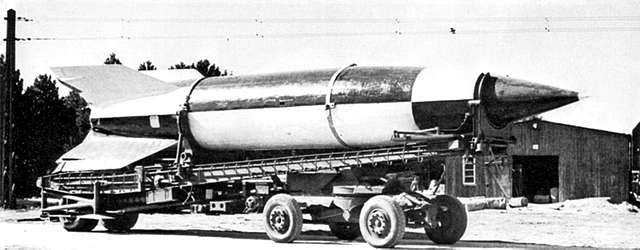
\includegraphics[width=0.75\linewidth]{figures/LiteratureStudy/V2_image.jpg}
    \caption{V2 rocket on Meillerwagen.\footnote{\url{https://timelessmoon.getarchive.net/media/v-2-rocket-on-meillerwagen-9effc8} (Accessed: 22 May 2025)}}
    \label{fig:V2_rocket}
\end{figure}

During the subsonic regime, under Mach 0.8, the drag is independent of the Mach number as compressibility effects are minimal. The lift coefficient has an initial increase with Mach number before a decrease, with the magnitude of the change observed being greater at higher angles of attack as the circulation around the rocket increases.

For the transonic regime, between Mach 0.8 and 1.2, shock waves begin to form and propagate over the rocket's surface, causing \textit{drag divergence}. Resulting in a rapid rise in drag approaching maximum drag and lift at 1.2. Strong shock and boundary layer interactions cause unsteady flow inducing the coefficient's rise.

\begin{figure}[H]
    \centering
    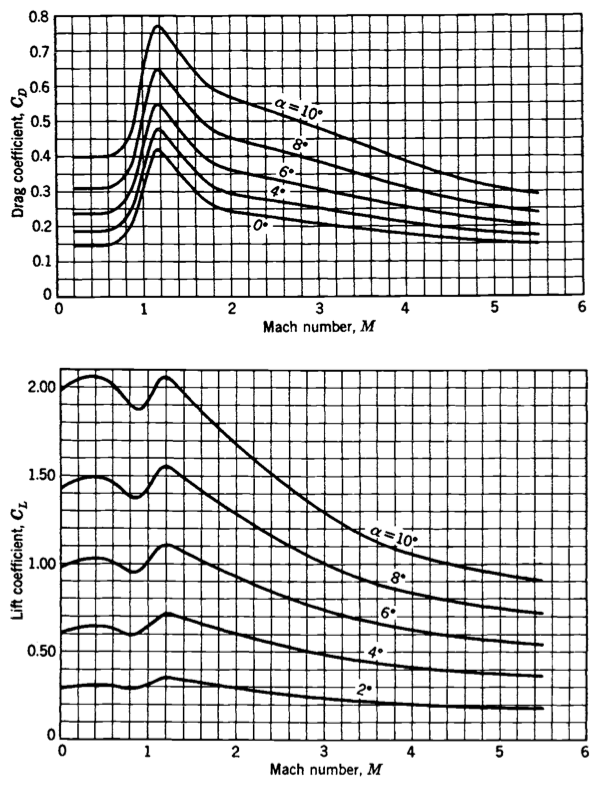
\includegraphics[width=0.75\linewidth]{figures/LiteratureStudy/V2-lift-drag-coefficient (1) (2).png}
    \caption{V2 rocket lift and drag coefficient curves (\cite{sutton_rocket_2016}).}
    \label{fig:V2_curves}
\end{figure}

The center of pressure (CoP) is the point on the rocket's body where the resultant aerodynamic force acts, in our case the lift and drag forces. \cite{TIR-33} states that a rocket during has aerodynamic stability if its center of pressure (CoP) is behind its center of gravity (CoG). A rocket may deviate for instance due to wind gusts, causing an increased angle of attack, a stable rocket will correct for this by forcing it back to zero over time. As a result, the center of pressure of the rocket is placed such that the rocket is aerodynamically stable during ascent and descent. A higher fidelity model for the center of pressure is not considered, as data on the V2 missile's center of pressure change with angle of attack and Mach number was not found. So the chosen CoP model cannot be validated, a constant center of pressure is taken.

The lift and drag coefficients of \autoref{fig:V2_curves} are converted to forces, lift and drag, through \autoref{eq:lift_drag}. Where the area $S$ is the cross-sectional area of the rocket, so $S = \pi \cdot r_r^2$, and the dynamic pressure is $q = \frac{1}{2} \cdot \rho \cdot V^2$.

\begin{equation}
\begin{aligned}
    L =& \frac{1}{2} \cdot \rho \cdot V^2 \cdot C_L \cdot S \\
    D =& \frac{1}{2} \cdot \rho \cdot V^2 \cdot C_D \cdot S
\end{aligned}
\label{eq:lift_drag}
\end{equation}

For the ascent phase, the center of pressure is behind the center of gravity, this gives the freebody diagram \autoref{fig:aero_reference_frames}, with angle of attack $\alpha$ the difference between the pitch and the flight path angle. Here two frames are present $(x',y')$ which is the initial reference frame, which is launchpad reference frame; x horizontal and right upward, translated to act at the rocket's center of gravity.$(x'',y'')$ is the body frame. From this freebody diagram the equations of motion can be derived, \autoref{eq:aero_forces_ascent}.

\begin{equation}
\begin{aligned}
    F_{x''} =& -L \cdot \cos(\alpha) -D\cdot\sin(\alpha) \\
    F_{y''} =& L \cdot \sin(\alpha) - D \cdot \cos(\alpha) \\
    M_z =& (d_{cg} - d_{cp}) \cdot ( -L \cdot \cos(\alpha) -D\cdot\sin(\alpha))
\end{aligned}
\label{eq:aero_forces_ascent}
\end{equation}

The center of pressure location is checked to find it's stable position with respect to the center of gravity. When an angle of attack is formed a negative aerodynamic moment is desired to correct the angle of attack. \autoref{eq:stability_ascent} derives the moments derivative with respect to angle of attack, before applying the small angle approximation. With a small $\alpha$ then $L\cdot \alpha << D$, and with the rest of the factors positive, the moment is restored.

\begin{equation}
\begin{aligned}
    \frac{dM_z}{d\alpha} =& (d_{cp} - d_{cg}) \cdot (L \cdot \sin(\alpha) -D \cdot \cos(\alpha) - C_{L_\alpha} q \cdot S\cdot \cos(\alpha) - C_{D_\alpha} \cdot q \cdot S \sin(\alpha)) \\
    =& (d_{cp} - d_{cg}) \cdot (L \cdot \alpha - D - C_{L_\alpha}\cdot q \cdot S - C_{D_\alpha} \cdot q \cdot S \cdot \alpha)
\end{aligned}
\label{eq:stability_ascent}
\end{equation}

The descent reference from of \autoref{fig:aero_reference_frames} is used to derive the body frame forces from the aerodynamics in \autoref{eq:descent_aero}. The effective angle of attack denotes the descent angle of attack which is found using \autoref{eq:eff_alpha}.

\begin{equation}
    \alpha_{eff} = \gamma - (\theta + \pi)
\label{eq:eff_alpha}
\end{equation}
        
\begin{equation}
\begin{aligned}
    F_{x''} =& -D \cdot \sin(\alpha_{eff}) - L \cdot \cos(\alpha_{eff}) \\
    F_{y''} =& D \cdot \cos(\alpha_{eff}) - L \cdot \sin(\alpha_{eff}) \\
     M_z =& (d_{cg} - d_{cp}) \cdot( -D \cdot \sin(\alpha_{eff}) - L \cdot \cos(\alpha_{eff}))
\end{aligned}
\label{eq:descent_aero}
\end{equation}

With the center of pressure now moved to the top of the rocket, the aerodynamic stability is checked in \autoref{eq:stability_descent}. For aerodynamic stability a positive restoring moment is required to minimise the angle of a. \autoref{eq:stability_descent} derives the moment derivative with respect to effective angle of attack before the small angle approximation is applied. A small angle of will make $L \cdot \alpha_{eff} << D$ so the applied moment is positive, as the rest of the terms are positive.

\begin{equation}
\begin{aligned}
    \frac{dM_z}{d\alpha_{eff}} =& (d_{cp} - d_{cg}) \cdot (C_{D_{\alpha_{eff}}} \cdot q \cdot S \cdot \sin(\alpha_{eff}) + C_{L_{\alpha_{eff}}} \cdot q \cdot S \cdot \cos(\alpha_{eff}) + D \cdot \cos(\alpha_{eff}) - L \cdot \sin(\alpha_{eff})) \\
    =& (d_{cp} - d_{cp}) \cdot (C_{D_{\alpha_{eff}}} \cdot q \cdot S \cdot \alpha_{eff} + C_{L_{\alpha_{eff}}} \cdot q \cdot S + D - L \cdot \alpha_{eff})
\end{aligned}
\label{eq:stability_descent}
\end{equation}

The translate into the inertia frame the transformations of \autoref{eq:inertial_aero} are performed, for descent and ascent.

\begin{equation}
\begin{aligned}
    F_{x'} =& F_{y''} \cdot \cos(\theta) + F_{x''} \cdot \sin(\theta) \\
    F_{y'} =& F_{y''} \cdot \sin(\theta) - F_{x''} \cdot \cos(\theta)
\end{aligned}
\label{eq:inertial_aero}
\end{equation}    

\begin{figure}[H]
    \centering
    \begin{subcaptionbox}{Ascent.}[0.45\linewidth]
        {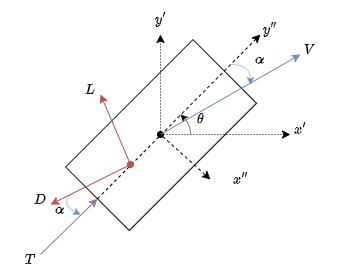
\includegraphics[width=\linewidth]{figures/LiteratureStudy/AerodynamicReference_ascent.png}}
        \label{fig:ascent_aero}
    \end{subcaptionbox}
    \hfill
    \begin{subcaptionbox}{Descent.}[0.45\linewidth]
        {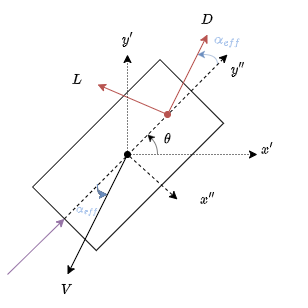
\includegraphics[width=\linewidth]{figures/LiteratureStudy/AerodynamicReference_descent (1).png} (1).png}
        \label{fig:descent_aero}
    \end{subcaptionbox}
    \caption{Aerodynamic Reference frames}
    \label{fig:aero_reference_frames}
\end{figure}

\subsection{Aerodynamic control surfaces}
\label{sec:ACS}
The aerodynamic control surfaces present on the rocket were chosen to grid fins in \autoref{sec:GNC}, as used on Space X's \textit{Super Heavy Booster}. Grid fins provide longitudinal and angular control, while also giving some drag to slow down the rocket. For Space X's electric motors torque the grid fins to their desired angle, as a result a first order low-pass filter can be used to model the lag in their actuation.

\cite{washington1993grid} perform experiments on grid fins and give curves for their drag and normal force coefficients, as these are validated examples of the change in aerodynamic coefficients for grid fins these shall be used as they provide a representative benchmark. The drag coefficient is roughly equal to the axial force coefficient of the grid fins at low angles of attack, as such \autoref{fig:drag_coeff_grid} can be interpolated by using \textit{WebPlotDigitiser} to extract points on the curve before linear interpolation. Washington also gives a curve for a curve for the change in the normal force coefficient with local angle of attack, \autoref{fig:cnalpha_grid}.

\begin{figure}[H]
    \centering
    \begin{subfigure}[b]{0.48\linewidth}
        \centering
        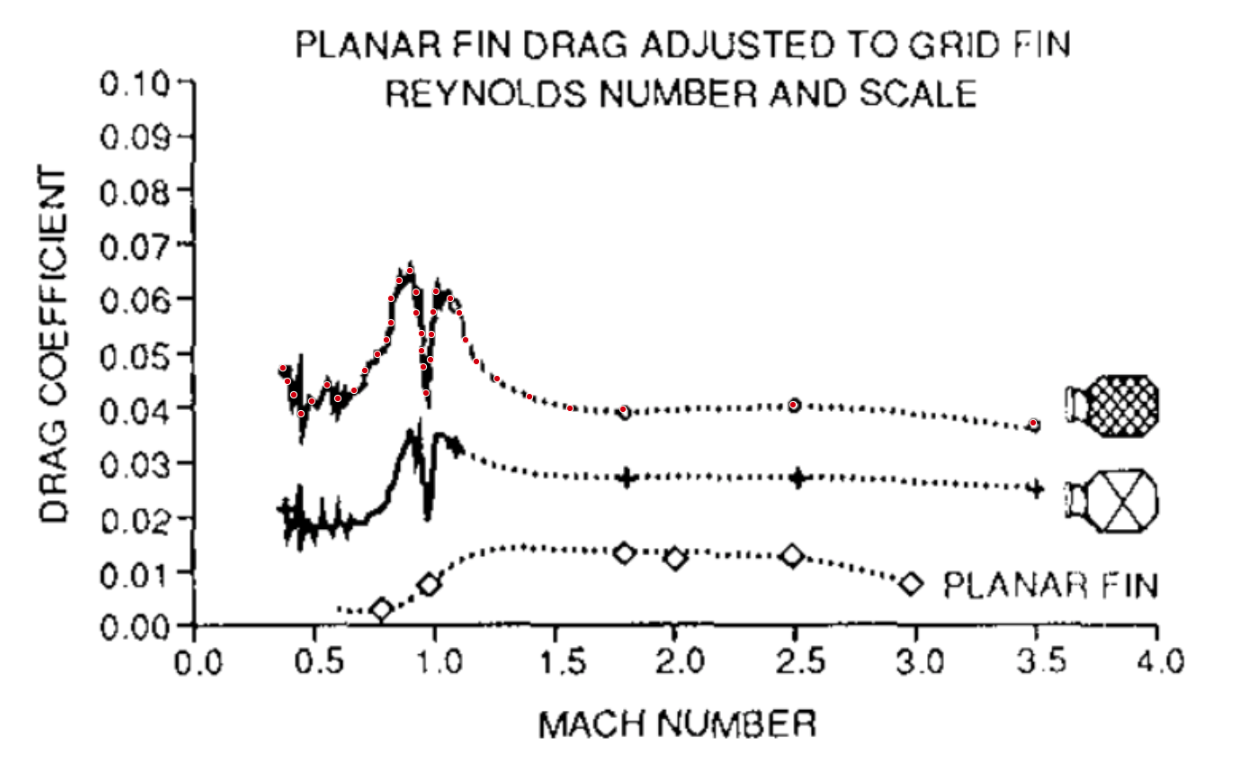
\includegraphics[width=\linewidth]{figures/LiteratureStudy/GridFins/DragCoefficientInterpolation.png}
        \caption{$C_D$ of a fin with points selected for interpolation \cite{washington1993grid}}
        \label{fig:drag_coeff_grid}
    \end{subfigure}
    \hfill
    \begin{subfigure}[b]{0.48\linewidth}
        \centering
        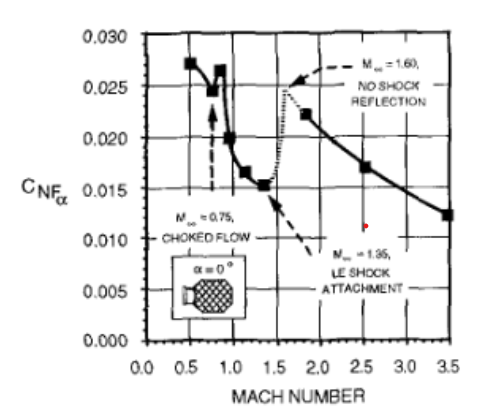
\includegraphics[width=\linewidth]{figures/LiteratureStudy/GridFins/CNGalpha_GF.png}
        \caption{$C_{N_\alpha}$ of a grid fin \cite{washington1993grid}}
        \label{fig:cnalpha_grid}
    \end{subfigure}
    \caption{Side-by-side comparison of drag coefficient and normal-force gradient for a grid fin}
    \label{fig:gridfin_side_by_side}
\end{figure}

The local angle of attack is the angle of the grid fin to the perpendicular direction of the flow. \autoref{eq:grid_fin_local_alpha} shows the local angle of attack for the left and right grid fins dependent on the effective angle of attack (descent angle of attack) and their respective deflection angles. The deflection angles go counter-clockwise, so an upward right grid fin deflection and a negative left grid fin deflection are positive.

\begin{equation}
\begin{aligned}
    \alpha_{l,R} =& \alpha_{eff} - \delta \\
    \alpha_{l,L} =& \alpha_{eff} + \delta 
\end{aligned}
\label{eq:grid_fin_local_alpha}
\end{equation}

With the angle of attack acting on each grid fin defined, the normal and axial force can be found from \autoref{fig:ACS_FBD}. First, the axial forces are the same for each grid fin as they are only dependent on Mach number. Second, the grid fins in the center of our 2D rocket are only modelled to give axial force as the third dimension is not considered.

\begin{equation}
\begin{aligned}
    F_a =& q \cdot S \cdot C_a(M) \\
    F_{N,L} =& q \cdot S \cdot C_n(M,\alpha_{l,L}) \\
    F_{N,R} =& q \cdot S \cdot C_n(M,\alpha_{l,R}) \\
\end{aligned}
\label{eq:grid_fin_aero_forces}
\end{equation}

The freebody diagram of the rocket during descent with grid fins is shown in \autoref{fig:ACS_FBD}. From this the perpendicular and parallel (x'', y'') forces are derived in \autoref{eq:ACS_para_perp}.

\begin{figure}[H]
    \centering
    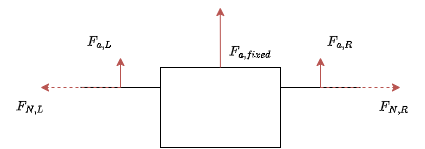
\includegraphics[width=0.5\linewidth]{figures/LiteratureStudy/GridFins/ACS_simple.png}
    \caption{Aerodynamic Control Surfaces freebody diagram during descent.}
    \label{fig:ACS_FBD}
\end{figure}

\begin{equation}
\begin{aligned}
    F_{x''} =& F_a \cdot (\cos(\delta_R) - \cos(\delta_L)) -F_{N,L} \cdot \cos(\delta_L) + F_{N_R} \cdot \cos(\delta_R) \\
    F_{y''} =& F_a \cdot (2 + \sin(\delta_L) + \sin(\delta_R)) - F_{N,L} \cdot \cos(\delta_L) + F_{N,R} \cdot \cos(\delta_R) \\
    M_z =& -(d_{gf}-d_{cg}) \cdot \bigg(F_a \cdot (\cos(\delta_R) - \cos(\delta_L)) -F_{N,L} \cdot \cos(\delta_L) + F_{N_R} \cdot \cos(\delta_R)\bigg) \\&+ r_r \cdot \bigg(F_{a} \cdot(\sin(\delta_R)-\sin(\delta_L) )+ F_{N,R} \cdot \cos(\delta_R) + F_{N,L} \cdot \cos(\delta_L)\bigg)
\end{aligned}
\label{eq:ACS_para_perp}
\end{equation}



\subsection{Atmosphere}
\label{sec:Atmosphere}
% ISA
% Gravity

Atmosphere dynamics influence the trajectory of the rocket, and the as such the control system design. Robust control systems need to adapt to disturbances and uncertainties, for instance wind in our case causing changes in relative velocities. Turbulence models, gusts, are often in the form of Dryden and von Karman models.

\cite{Mulder2020} state that the von Karman spectral densities are not rational functions, as such the Dryden model was introduced. However, the von Karman form does align better with experimental data, the Dryden form generally causes similar aircraft responses, as such the Dryden models shall be used.

Variations in relative velocity, caused by wind gusts, introduce dynamic changes that the control system must counteract in real time. Modelling these variations ensures a robust control strategy can be created to withstand them

As for atmosphere models, the International Standard Atmosphere (ISA) model is taken from \cite{Anderson2020Introduction}, and gravitational acceleration is calculated using \autoref{eq:grav}.

\begin{equation}
    g = g_0 \cdot \bigg(\frac{R_{E}}{R_{E} + y}\bigg)^2
\label{eq:grav}
\end{equation}


\subsection{Rocket engines}
\label{sec:RocketEngines}
The rocket engines provide the main source of acceleration to the rocket. Each engine/thruster is assumed to have identical throttle, and the gimballed thrusters identical gimbal angles, as explained in \autoref{sec:GNC} to limit the size of the action space for this benchmark study. To improve the simulation fidelity pressure losses have been included through \autoref{eq:pressure_losses}, because as the rocket moves through the atmosphere the atmospheric pressure will change altering the true thrust the thrusters enact on the rocket.

As the rocket burns propellant, fuel and oxidiser, will be consumed changing the mass of the rocket with the mass flow linearly scaled with throttle. Furthermore, a minimum of 40\% throttle per thruster has been enacted to keep inline with available thrusters. However, during descent the number of rocket engines active will decrease, this switching isn't modelled, but the central three thruster's are assumed always active as seen with the Super Heavy booster.

% Gimballing
The gimbal angle is defined as counter-clockwise to keep conventions uniform, this gives the body frame force's from the thrusters in \autoref{eq:thrust_ref}, with \autoref{eq:inertial_aero} providing the inertial frame translation.

\begin{equation}
\begin{aligned}
    F_{x''} =& - T^g \cdot \sin(\theta^g) \\
    F_{y''} =& T^{ng} + T^g \cdot \cos(\theta^g) \\
    M_z =& -(d_{cg} - d_{t}) T^g \cdot \sin(\theta^g)
\end{aligned}
\label{eq:thrust_ref}
\end{equation}

\subsection{Equations of motion}
\label{sec:EoM}
The previous subsections of this section has sized the rocket, and enacted forces upon the rocket. Here these will be collated together to form equations of motion for the rocket. The forces applied to the rocket are the some of the enacting forces in their respective axes. These forces come from the ACS, aerodynamics, thrusters and gravity, also apply moments to the body asides from gravity, with the RCS's cold gas thrusters applying a pure moment aswell when activated.

Newton's 2nd law, \autoref{eq:Netwons2nd}, converts the forces into the rocket's acceleration. The explicit first-order forward Euler numerical integration scheme is used to integrate acceleration into velocity and then position, as it offers a computationally inexpensive and easy to implement approach adequate for a low-fidelity simulation with a small time constant of 0.1 seconds.

\begin{equation}
    F= m \cdot a \rightarrow \ddot{x} = a = \frac{F}{m}
\label{eq:Netwons2nd}
\end{equation}

Euler's rotational motion equation, \autoref{eq:Euler_rotational}, is used to enact the moment's change on the orientation (pitch) of the rocket. The inertia changes and is updated as fuel is consumed, the model for derived for this inertia change is shown in \autoref{sec:inertia}. Again a explicit first-order forward Euler numerical integrations scheme is used.

\begin{equation}
    \ddot{\theta} = \frac{M}{I}
\label{eq:Euler_rotational}
\end{equation}

\chapter{Additional Results}
\label{chp:additional_results}
\section{Staging verification}
\label{sec:staging_verification}

% Verification to paper's parameters
The verify the implementation it was compared to results of \cite{ReusbaleStaging} as documented in Table 1 through their optimal configuration. However, there will be discrepancies, as the velocity loss and descent increments are found after the configuration is build, as documented in \autoref{tab:Comparsions}. As a result, intermediate verification steps can take place, but the full results will not be identical. This can be proven as the when putting these values in and reverse calculating from the final reusable and expendable step gives different $\kappa$ values.

\begin{table}[H]
    \centering
    \caption{Comparison of result to \cite{ReusbaleStaging}.}
    \begin{tabular}{|c|c|c|c|}
    \hline
        Value & \cite{ReusbaleStaging} & Reproduction & Difference (\%) \\ \hline
        Take-off mass [t] & 555.6 & 863.8 & 55 \\
        Structural mass stage 1 [t] & 21.5 & 34.6 & 61 \\
        Structural mass stage 2 [t] & 5.7 & 8.4 & 45 \\
        Propellant mass stage 1 [t] & 398.6 & 641.4 & 60 \\
        Propellant mass stage 2 [t] & 114.2 & 163.8 & 43 \\
        Payload ratio stage 1 [\%] & 32.3 & 28 & 13 \\
        Payload ratio stage 2 [\%] & 12.9 & 9 & 30 \\
        Optimal loss-free stage 1 ascent $\Delta v$ [$m/s$] & 1799 & 1454.6 & -19 \\
        Optimal loss-free stage 2 $\Delta v$ [$m/s$] & 5600 & 6323.8 & 13 \\ \hline
    \end{tabular}
    \label{tab:Comparsions}
\end{table}

Step-by-step verification was conducted reversing their equations caused a $\kappa$ of approximately 2555 needed to get the reusable stage desired values, from the losses given, but a $\kappa$ of 2693.0 is needed to get the expendable stage's desired values. As a result, \autoref{tab:Comparsions} will not produce the same values, as the velocity increments used for sizing are different to the velocity losses from the trajectory optimiser.

First, for expendable stage, from rearranging \autoref{eq:masses_expendable} \autoref{eq:stage_verif_1} can be found. The resulting payload ratio of 12.9 aligns with their results.

\begin{equation}
    \lambda_2^{l^*} = \frac{m_{pay}}{m_2} = \frac{m_{pay}}{m_{s,2} + m_{p,2}} = \frac{15.5e3}{5.7e3 + 114.2e3} = 0.12927
\label{eq:stage_verif_1}
\end{equation}

Second, the velocity increment needed is derived in \autoref{eq:stage_verif_2} from \autoref{eq:payload_opt_losses}. 

\begin{equation}
    \Delta v_2 = \Delta v_2^* - \Delta v_{loss,2} = v_{ex,2} \cdot \ln(\frac{\lambda_2^{l^*}  + 1}{\lambda_2^{l^*}  + \epsilon_2}) = 3412 \cdot \ln(\frac{0.129 + 1}{0.129 + 4.867e-3}) = 6309.3
\label{eq:stage_verif_2}
\end{equation}

The corresponding optimal loss-free velocity increment for the second stage, is then correct, according to their values.

\begin{equation}
\begin{aligned}
    \Delta v_2^* =  \Delta v_2 - \Delta v_{loss,2} = 6309.2 - 710 \approx 5600
\end{aligned}
\label{eq:stage_verif_3}
\end{equation}

Rearranging the Tsiolkovsky equation of \autoref{eq:Tsiolkovsky} to find the optimal loss-free payload ratio give \autoref{eq:stage_verif_4}.

\begin{equation}
    \lambda_2^* = \frac{1 - \epsilon_2 \cdot e^{\frac{\Delta v^*_2}{v_{{ex,2}}}}}{e^{\frac{\Delta v^*_2}{v_{ex,2}}} - 1} = 0.1799
\label{eq:stage_verif_4}
\end{equation}

Then rearranging \autoref{eq:payload_opt} to find $\kappa$, producing a $\kappa$ different to the one found in the reproduction of 2352.

\begin{equation}
    \kappa = \frac{\lambda_2^* \cdot (1 - \epsilon_2) \cdot v_{ex,2}}{\epsilon_2 + \lambda_2^*} = 2555.8
\label{eq:stage_verif_5}
\end{equation}

On the other, hand looking at the reusable stage by rearranging \autoref{eq:opt_payload_reusable} and \autoref{eq:velocity_incrmenet_1} to get \autoref{eq:stage_verif_5} shows how the $\kappa$ differs from that calculated for the expendable stage.

\begin{equation}
\begin{aligned}
    \lambda_1^* =& \frac{1 - e^{\frac{\Delta v_{a,1}^*}{v_{ex,1}}} \cdot \epsilon_{a,1}}{e^{\frac{\Delta v_{a,1}^*}{v_{ex,1}}} - 1} = 0.9253 \\
    \kappa =& \frac{\lambda_1^* \dot (1 - \epsilon_{a,1}) \cdot v_{ex,1}}{\epsilon_{a,1} + \lambda_1^*} = 2268.27
\end{aligned}
\label{eq:stage_verif_5}
\end{equation}

% TODO: Step-by-step verification

\begin{table}[H]
    \centering
    \begin{minipage}{0.45\textwidth}
        \centering
        \caption{Staging inputs}
        \begin{tabular}{|c|c|}
             \hline
             Variable [unit] & Value \\ \hline
             \hline
        \end{tabular}
        \label{tab:staging_inputs}
    \end{minipage}%
    \hspace{0.05\textwidth}
    \begin{minipage}{0.45\textwidth}
        \centering
        \caption{Staging results}
        \begin{tabular}{|c|c|c|}
            \hline
             Variable [unit] & Stage 1 & Stage 2 \\ \hline
             $m_{s_a}$ [t] & - & - \\
             $m_{p_a}$ [t] & - & - \\
             $m_{s_d}$ [t] & - & - \\
             $m_{p_d}$ [t] * - & - \\
        \end{tabular}
        \label{tab:staging_results}
    \end{minipage}
\end{table}

% TODO: Comparison to Space X values.


\section{Inertia determination}
\label{sec:inertia}

As the rocket burns fuel the fill level of the tanks will decrease resulting in a change of center of gravity and inertia. To model this affect, functions for each of the subrocket are created to output the center of gravity and inertia as a function of fuel consumption. First, the rocket is sized and each independent stage's inertia and center of gravity of functions are found, then combined for the subrockets.

\textbf{Tank sizing}: the tanks are sized assuming cylindrical tanks, the constants of \autoref{tab:tank_sizing_constants} are used in \autoref{eq:tank_sizing} to give the height of tanks and the mass of the fluid within them. The results are displayed in \autoref{tab:tank_sizing_results}.

\begin{equation}
\begin{aligned}
    m_{LOX} =& \frac{m_{prop}}{\frac{O}{F}} \\
    m_{LCH_4} =& m_{prop} - m_{LOX} \\
    h_f =& \frac{m_{LCH_4}}{\rho_{LCH_4}} \cdot \frac{1}{\pi \cdot (r_r - t_{wall})^2} \\
    h_{ox} =& \frac{m_{LOX}}{\rho_{LOX}} \cdot \frac{1}{\pi \cdot (r_r - t_{wall})^2}
\end{aligned}
\label{eq:tank_sizing}
\end{equation}

\begin{table}[H]
    \centering
    \begin{minipage}{0.45\textwidth}
        \centering
        \caption{Tank sizing constants}
        \begin{tabular}{|c|c|}
             \hline
             Variable [unit] & Value \\ \hline
             $\rho_{LOX}$ [$kg/m^3$] & 1200 \\
             $\rho_{LCH_4}$ [$kg/m^3$] & 450 \\
             $\frac{O}{F}$ [$-$] & 3.545 \\
             $t_{wall}$ [$m$] & 0.01 \\
             \hline
        \end{tabular}
        \label{tab:tank_sizing_constants}
    \end{minipage}%
    \hspace{0.05\textwidth}
    \begin{minipage}{0.45\textwidth}
        \centering
        \caption{Tank sizing results}
        \begin{tabular}{|c|c|c|}
            \hline
             Variable [unit] & Stage 1 & Stage 2 \\ \hline
             $m_{LOX}$ [$kg$] & - & - \\
             $m_{LCH_4}$ [$kg$] & - & - \\
             $h_{LOX}$ [$m$] & - & - \\
             $h_{LCH_4}$ [$m$] & - & - \\ \hline
        \end{tabular}
        \label{tab:tank_sizing_results}
    \end{minipage}
\end{table}

\textbf{Stage sizing procedure}

The 2 stage rocket was divided into sections, as shown in \autoref{fig:rocket_sections} to determine the center of gravity and inertia through low fidelity sizing. This is not an accurate, however is representative of change in inertia a rocket might experience. The first stage has four structural mass components, a lower and upper section containing avionics equipment, stage and engine adapters, and the tank's structural walls and engines themselves. The second stage replaces has an additional payload and nose section.

\begin{figure}[H]
    \centering
    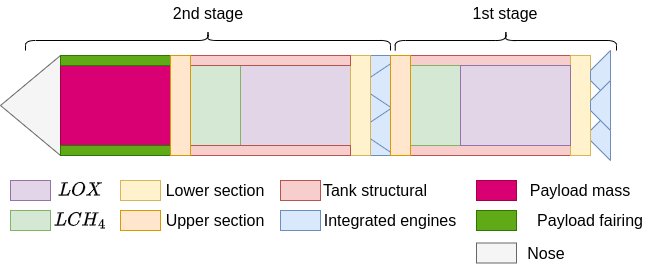
\includegraphics[width=0.95\linewidth]{figures/LiteratureStudy/RocketDiagram_new_new.png}
    \caption{Sectioning of rocket}
    \label{fig:rocket_sections}
\end{figure}

\textbf{First stage dry inertia}: The masses of each of the first stage are calculated through \autoref{eq:stage_masses_1}, using cylindrical tanks. The $\Lambda_{ul}$ is the factor of mass remaining structural mass distribution between the upper and lower section height.

\begin{equation}
\begin{aligned}
    m_{s,tanks} =& \pi \cdot (h_f + h_{ox}) \cdot (r_r^2 - (r_r - t_{wall})^2) \cdot \rho_{304L} \\
    m_{e,stage} =& n_e \cdot m_{e,integrated} \\
    m_{upper} =& (m_s - m_{s,tanks} - m_{e,stage}) \cdot \frac{1}{1 + \Lambda_{ul}} \\
    m_{lower} =& (m_s - m_{s,tanks} - m_{e,stage}) \cdot \frac{\Lambda_{ul}}{1+\Lambda_{ul}}
\end{aligned}
\label{eq:stage_masses_1}
\end{equation}

\begin{equation}
\begin{aligned}
    h_{upper} =& \frac{m_{upper}}{\rho_{upper}} \cdot \frac{1}{\pi \cdot r_r^2} \\
    h_{lower} =& \frac{m_{lower}}{\rho_{lower}} \cdot \frac{1}{\pi \cdot r_r^2} \\
\end{aligned}
\label{eq:section_heights}
\end{equation}

\begin{equation}
    x_{dry} = \frac{-m_{e,stage} \cdot \frac{h_e}{2} + m_{lower} \cdot \frac{h_{lower}}{2} + m_{s,tanks} \cdot (h_{lower} + \frac{h_f + h_{ox}}{2}) + m_{upper} \cdot (h_{lower} + h_f + h_{ox} + \frac{h_{upper}}{2})}{m_s}
\label{eq:dry_cog}
\end{equation}

Now the dry inertia is calculated using the cylinder moment of inertia equation

\begin{equation}
\begin{aligned}
    I_{e,stage} =& \frac{1}{12} \cdot m_{e,stage} \cdot h_e^2 - m_{e,stage} \cdot (x_{dry} + \frac{h_e}{2})^2 \\
    I_{lower} =& \frac{1}{12} \cdot m_{lower} \cdot h_{lower}^2 + m_{lower} \cdot (\frac{h_{lower}}{2} - x_{dry})^2 \\
    I_{upper} =& \frac{1}{12} \cdot m_{upper} \cdot h_{upper}^2 + m_{upper} \cdot (h_{lower} + h_{ox} + h_f + \frac{h_{upper}}{2} - x_{dry})^2 \\
    I_{s,tanks} =& \frac{1}{12} \cdot m_{s,tanks} \cdot (h_f + h_{ox})^2 + m_{s,tanks} \cdot (h_{lower} + \frac{h_f + h_{ox}}{2} - x_{dry})^2 \\
    I_{dry} =& I_{e,stage} + I_{lower} + I_{upper} + I_{s,tanks}
\end{aligned}
\label{eq:dry_inertia_1}
\end{equation}

\textbf{Second stage dry moment of inertia}: The payload structural mass is first computed using \autoref{eq:payload_strc}, alike to the tank structural masses. \autoref{eq:stage_masses_1} is used to get the stage's total integrated engines mass, and the tank structural mass. Using the volume of cone the nose mase is calculated in \autoref{eq:dry_2} allowing for the left-over mass to be applied to the second stage's lower and stages.

\begin{equation}
\begin{aligned}
    h_{pay} =& \frac{m_{pay}}{\rho_{pay}} \cdot \frac{1}{\pi \cdot (r_r - t_{fairing})^2} \\
    m_{s,pay} =& \pi \cdot h_{pay} \cdot (r_r^2 - (r_r - t_{fairing})^2) \cdot \rho_{304L}
\end{aligned}
\label{eq:payload_strc}
\end{equation}

\begin{equation}
\begin{aligned}
    m_{s,nose} =& \frac{1}{3} \cdot \pi r_r^3 \cdot \rho_{nose}\\
    m_{s,upper} =& (m_s - m_{s,pay} - m_{s,tanks} - m_{e,stage} - m_{s,nose}) \cdot \frac{1}{1 + \Lambda_{ul}}\\
    m_{s,lower} =& (m_s - m_{s,pay} - m_{s,tanks} - m_{e,stage} - m_{s,nose}) \cdot \frac{\Lambda_{ul}}{1 + \Lambda_{ul}}\\
\end{aligned}
\label{eq:dry_2}
\end{equation}

The dry center of gravity for the second stage including payload mass becomes:

\begin{equation}
\begin{aligned}
    x_{cog} =& [-m_{e,stage} \cdot \frac{h_e}{2} + m_{lower} \cdot \frac{h_{lower}}{2} + m_{s,tank} \cdot (h_{lower} + \frac{h_f + h_{ox}}{2}) \\
    +& m_{upper} \cdot (h_{lower} + h_f + h_{ox} + \frac{h_{upper}}{2}) + (m_{pay} + m_{s,pay}) \cdot (h_{lower} + h_f + h_{ox} + h_{upper} +  \frac{h_{pay}}{2}) \\
    +& m_{nose} \cdot (h_{lower} + h_f + h_{ox} + h_{upper} + h_{pay} + \frac{r_r}{8}] \cdot \frac{1}{m_s + m_{pay}}
\end{aligned}
\end{equation}


Now the dry moment of inertia can be found, taking $I_{e,stage}$, $I_{lower}$, $I_{upper}$ and $I_{s,tanks}$ from \autoref{eq:dry_inertia_1}.

\begin{equation}
\begin{aligned}
    I_{pay} =& \frac{1}{12} \cdot (m_{pay} + m_{s,pay}) \cdot  h_{pay}^2 + (m_{pay} + m_{s,pay}) \cdot (h_{lower} + h_f + h_{ox} + h_{upper} + \frac{h_{pay}}{2} - x_{dry})^2 \\
    I_{nose} =& \frac{3}{80} \cdot m_{s,nose} \cdot (5 \cdot r_r^2) + m_{s,nose} \cdot (h_{lower} + h_f + h_{ox} + h_{upper} + h_{pay} + \frac{r_r}{4} - x_{dry})^2 \\
    I_{dry} =& I_{e,stage} + I_{lower} + I_{upper} + I_{s,tanks} + I_{pay} + I_{nose}
\end{aligned}
\label{eq:dry_inertia_2}
\end{equation}

\textbf{Wet center of gravity}. As propellant is consumed the center of gravity of the propellant will shift towards the rocket, as modelled by \autoref{eq:prop_x_cog}.

\begin{equation}
    x_{prop} = \frac{m_{ox} \cdot (h_{lower} + \frac{h_{ox}}{2}) + m_f \cdot (h_{lower} + h_{ox} + \frac{h_f}{2})}{m_{prop}}
\label{eq:prop_x_cog}
\end{equation}

\begin{equation}
\begin{aligned}
    x_{wet,1} =& \frac{x_{dry,1} \cdot m_{s,1} + x_{prop,1} \cdot m_{prop,1}}{m_{s,1} + m_{prop,1}} \\
    x_{wet,2} =& \frac{x_{dry,2} \cdot (m_{pay} + m_{s,2}) + x_{prop,2} \cdot m_{prop,2}}{m_{s,2} + m_{prop,2} + m_{pay}}
\label{eq:wet_cog}
\end{aligned}
\end{equation}

\textbf{Wet moment of inertia}: As said before as propellant is consumed the inertia and center of gravity of wet mass will change

\begin{equation}
\begin{aligned}
    \tilde{h}_{ox} =& h_{ox} \cdot f^l \quad &\tilde{h}_f = h_f \cdot f^l \\
    \tilde{m}_{ox} =& m_{ox} \cdot f^l \quad &\tilde{m}_f = m_f \cdot f^l \\
\end{aligned}
\end{equation}

\begin{equation}
    \tilde{x}_{prop} = \frac{\tilde{m}_{ox} \cdot (h_{lower} + \frac{\tilde{h_{ox}}}{2}) + \tilde{m}_f \cdot (h_{lower} + h_{ox} + \frac{\tilde{m}_f}{2})}{\tilde{m}_{ox} + \tilde{m}_f}
\end{equation}

Inertia in the tank frame then becomes...

\begin{equation}
\begin{aligned}
    \tilde{I}_{ox} =& \frac{1}{12} \cdot \tilde{m}_{ox} \cdot \tilde{h}_{ox}^2 + \tilde{m}_{ox} \cdot (h_{lower} + \frac{\tilde{h}_{ox}}{2} - \tilde{x}_{prop})^2 \\
    \tilde{I}_{f} =& \frac{1}{12} \cdot \tilde{m}_f \cdot \tilde{h}_f^2 + \tilde{m}_f \cdot (h_{lower} + h_{ox} + \frac{\tilde{h}_f}{2})^2 \\
    \tilde{I}_{prop} =& \tilde{I}_{ox} + \tilde{I}_f
\end{aligned}
\end{equation}

The wet center of gravity is then updated

\begin{equation}
    \tilde{x}_{wet} = \frac{m_s \cdot x_{dry} + \tilde{m}_{prop} \cdot \tilde{x}_{prop}}{m_{dry} + \tilde{m}_{prop}}
\end{equation}

This results in a wet moment of inertia of

\begin{equation}
\begin{aligned}
    \hat{I}_{dry} =& I_{dry} + m_{s} \cdot (x_{dry} - \tilde{x}_{wet})^2 \\
    \hat{I}_{prop} =& I_{prop} + \tilde{m}_{prop} \cdot (\tilde{x}_{prop} - \tilde{x}_{wet})^2 \\
    \hat{I}_{stage} =& \hat{I}_{dry} + \hat{I}_{prop}
\end{aligned}
\end{equation}

\textbf{Full rocket inertia:} before stage separation both stages travel together, so there centers of gravity and inertias must be collated together.

\begin{equation}
    \tilde{x}_{rocket} = \frac{m_{s,1} \cdot x_{dry,1} + (m_2 + m_{pay}) \cdot (x_{wet,2} + h_1) + \tilde{m}_{prop,1} \cdot \tilde{x}_{prop,1}}{m_{s,1} + m_{2} + m_{pay} + \tilde{m}_{prop,1}}
\end{equation}

\begin{equation}
\begin{aligned}
    \hat{I}_{rocket} =& I_{dry,1} + I_{2} + I_{prop,1} + m_{s,1} \cdot (x_{dry,1} - \tilde{x}_{rocket})^2 \\
    &+ (m_{pay} + m_2) \cdot (h_1 + x_{wet,2} - \tilde{x}_{rocket})^2 + \tilde{m}_{prop,1} \cdot (\tilde{x}_{prop,1} - \tilde{x}_{rocket})^2
\end{aligned}
\end{equation}

\section{Aerodynamic stability}
\label{sec:AerodynamicStability}
\input{mainmatter/AdditionalResults/4_AerodynamicStability}

\chapter{Conclusion}
\label{chp:conclusion}


\section{Conclusion}
\label{sec:conclusion}

\section{Recommendations}
\label{sec:recommendations}


%% Prevent urls running into margins in bibliography
\setcounter{biburlnumpenalty}{7000}
\setcounter{biburllcpenalty}{7000}
\setcounter{biburlucpenalty}{7000}

%% Add bibliography
\printbibliography[heading=bibintoc,title=References]

%% ----------------------------------------------------------------------
%%    Appendix (Letters for chapters)
%% ----------------------------------------------------------------------

\appendix
\chapter{Appendix}
\label{app:appendix}
\section{Programming specifications}
\label{sec:programming_defs}

The programming language shall be Python, with \texttt{JAX} as the chosen machine-learning library. Secondly, \texttt{gymnasium} by OpenAI shall wrap the environment. The PEP 8 \footnote{\url{https://peps.python.org/pep-0008/}. Accessed 09-12-2024.} coding style shall be used. Also, a \texttt{conda} environment will be used to manage dependencies, creating a \texttt{requirements} \texttt{.txt} or \texttt{.yaml} file to ease reproducibility. The \texttt{CUDA} framework for NVIDIA GPU acceleration shall be used, with the code being used on a Windows OS. GitHub will control the version, and VSCode will be the chosen IDE software. However, it will be compatible with all IDE software. Finally, the verification testing will use the testing framework called \texttt{PyTest}. The directory structure shall follow \autoref{fig:directory_structure}.

Data generated from results is not expected to be of large file size and, as such, shall be uploaded to the GitHub repository under the folders as specified in \autoref{fig:directory_structure}; so becomes open-sourced and readily available for reproducibility and repeatability studies. A separate \texttt{.md} file shall include an overview of the data. Finally, the codebase will be licensed through the Apache License, Version 2.0\footnote{\url{https://www.apache.org/licenses/LICENSE-2.0.html}. Accessed 09-12-2024.} to keep the data openly available.

\begin{figure}[H]
    \centering
    \begin{verbatim}
    project-root/
    │
    ├── src/                      # Project's source code
    │   ├── envs/                 # Custom environments, including Gymnasium wrappers
    │   ├── agents/               # RL agents
    │   ├── controllers/          # Controllers, ready to be incorporated with 
    │   ├──                         the environment; RL, MPC, etc.
    │   ├── utils/                # Utility functions, like logging and plotting
    │   ├── data_processing/      # Pre and post-processing scripts.
    │   └── main.py               # File to run the project
    │
    ├── tests/                    # Testing directory
    │   ├── unit/                 # Unit tests
    │   ├── system/               # System tests
    │   ├── validation/           # Validation tests
    │   └── test_main.py          # Script to run all tests
    │
    ├── data/                     # Directory for all data
    │   ├── raw/                  # Raw data files (.csv)
    │   ├── processed/            # Processed data files (.csv)
    │   ├── agents/               # Saved RL agents (.pth)
    │
    ├── notebooks/                # Jupyter notebooks for running specific 
    ├──                             experiments (all sub-files are .ipynb).
    │
    ├── docs/                     # Documentation
    │
    ├── configs/                  # Configuration files
    │   ├── model_parameters.py   # Simulation model parameters
    │   ├── agents_parameters.py  # Agent hyper-parameters  
    │   ├── other_parameters.py   # Other parameters  
    │
    ├── results/                  # Results and analysis outputs
    │   ├── figures/              # Plots and figures for reports
    │   ├── logs/                 # Logs
    │   └── reports/              # Generated reports or links ti them
    │
    ├── requirements.txt          # Dependencies
    ├── environment.yml           # Conda dependencies
    ├── .gitignore                # Git ignore
    └── README.md                 # Main README file for the project
    \end{verbatim}
    \caption{First draft of the directory structure for the rocket landing simulation project.}
    \label{fig:directory_structure}
\end{figure}

\end{document}
